% #53 DOI: 10.5281/zenodo.19616971

% ============================================================
% Paper #53 (Supplement)
% 0-Sphere Model Quartet Supplement: Papers #49, #50, #51, #52
% Preamble follows #54 (Hanamura 2026) convention
% ============================================================

\documentclass[12pt,letterpaper]{article}
\usepackage{amsmath,amssymb}
\usepackage{graphicx}
\usepackage{bm}
\usepackage{authblk}
\usepackage{setspace}
\usepackage{geometry}
\usepackage[labelfont=bf]{caption}

\usepackage{tabularx}
\usepackage{ragged2e}
\usepackage{booktabs}
\usepackage{longtable}
\usepackage{array}
\usepackage{enumitem}
\usepackage{xcolor}
\usepackage{tikz}
\usetikzlibrary{arrows.meta, positioning, calc, fit, backgrounds, shapes.geometric}
\usepackage{titlesec}
\usepackage{mdframed}
%\usepackage{microtype}
\usepackage{amsthm}
\usepackage[colorlinks=true,linkcolor=blue,citecolor=blue,urlcolor=blue]{hyperref}

\geometry{
  letterpaper,
  top=2.8cm,
  bottom=2.8cm,
  left=3.0cm,
  right=3.0cm
}

\onehalfspacing

\titleformat{\section}
  {\normalfont\large\bfseries}{\thesection}{1em}{}

\titleformat{\subsection}
  {\normalfont\normalsize\bfseries}{\thesubsection}{1em}{}

\titleformat{\subsubsection}
  {\normalfont\normalsize\itshape}{\thesubsubsection}{1em}{}

% ----- Color definitions (following #54) -----
\definecolor{threadblue}{RGB}{0,61,130}
\definecolor{threadgreen}{RGB}{26,107,58}
\definecolor{threadpurple}{RGB}{91,45,142}
\definecolor{threadred}{RGB}{160,30,30}
\definecolor{threadgray}{RGB}{90,90,90}
\definecolor{boxbg}{RGB}{245,248,255}
\definecolor{greenbg}{RGB}{238,247,240}
\definecolor{purplebg}{RGB}{243,238,249}
\definecolor{warningbg}{RGB}{255,248,230}
\definecolor{orangebg}{RGB}{253,243,227}

% ----- mdframed box styles -----
\mdfdefinestyle{bluebox}{
  backgroundcolor=boxbg,
  linecolor=threadblue,
  linewidth=2pt,
  leftline=true, rightline=false, topline=true, bottomline=true,
  leftmargin=0pt, rightmargin=0pt,
  innerleftmargin=12pt, innerrightmargin=10pt,
  innertopmargin=8pt, innerbottommargin=8pt
}
\mdfdefinestyle{greenbox}{
  backgroundcolor=greenbg,
  linecolor=threadgreen,
  linewidth=2pt,
  leftline=true, rightline=false, topline=true, bottomline=true,
  leftmargin=0pt, rightmargin=0pt,
  innerleftmargin=12pt, innerrightmargin=10pt,
  innertopmargin=8pt, innerbottommargin=8pt
}
\mdfdefinestyle{purplebox}{
  backgroundcolor=purplebg,
  linecolor=threadpurple,
  linewidth=2pt,
  leftline=true, rightline=false, topline=true, bottomline=true,
  leftmargin=0pt, rightmargin=0pt,
  innerleftmargin=12pt, innerrightmargin=10pt,
  innertopmargin=8pt, innerbottommargin=8pt
}
\mdfdefinestyle{chainbox}{
  backgroundcolor=boxbg,
  linecolor=threadblue,
  linewidth=1.5pt,
  leftline=true, rightline=true, topline=true, bottomline=true,
  leftmargin=20pt, rightmargin=0pt,
  innerleftmargin=14pt, innerrightmargin=10pt,
  innertopmargin=10pt, innerbottommargin=10pt
}
\mdfdefinestyle{orangebox}{
  backgroundcolor=orangebg,
  linecolor=orange!70!black,
  linewidth=2pt,
  leftline=true, rightline=false, topline=true, bottomline=true,
  leftmargin=0pt, rightmargin=0pt,
  innerleftmargin=12pt, innerrightmargin=10pt,
  innertopmargin=8pt, innerbottommargin=8pt
}
\mdfdefinestyle{openbox}{
  backgroundcolor=warningbg,
  linecolor=threadred,
  linewidth=1.5pt,
  leftline=true, rightline=false, topline=false, bottomline=false,
  leftmargin=0pt, rightmargin=0pt,
  innerleftmargin=12pt, innerrightmargin=10pt,
  innertopmargin=6pt, innerbottommargin=6pt
}

% ----- Convenience commands -----
\newcommand{\doilink}[1]{\texttt{#1}}
\newcommand{\paperno}[1]{\textbf{\#{}#1}}
\newcommand{\OmT}{\boldsymbol{\Omega}_T}
\newcommand{\vZB}{v_{\mathrm{ZB}}}
\newcommand{\lambdaC}{\lambda_{\mathrm{C}}}
\newcommand{\calS}{\mathcal{S}}
\newcommand{\calA}{\mathcal{A}}
\newcommand{\iphase}{\theta}
\newcommand{\anom}{a_{\mathrm{e}}}
\newcommand{\ehat}[1]{\hat{e}_{#1}}
\newcommand{\omZB}{\omega_{\text{ZB}}}
\newcommand{\betaZB}{\beta_{\mathrm{ZB}}}

% ----- Theorem environment -----
\newtheorem{theorem}{Theorem}[section]
\newtheorem{proposition}[theorem]{Proposition}

% ============================================================
\begin{document}
\sloppy
% ============================================================

\title{From Gravitational Mediation to Directional Force Classification:\\
\large A Conceptual and Mathematical Supplement to Papers \#49, \#50, \#51, and \#52 of the 0-Sphere Model Series\par\vspace{6pt}
{\normalsize Supplement Paper \#53}}

\author{Satoshi Hanamura\thanks{Email: hana.tensor@gmail.com}}
\date{April 19, 2026}

\maketitle

\tableofcontents
\clearpage

% ============================================================
\begin{center}
\textbf{\large Purpose and Reading Guide}
\end{center}
\justifying

\noindent This document is a conceptual and mathematical supplement to four research papers
in the 0-Sphere Model series:
\begin{itemize}[leftmargin=2em]
  \item \paperno{49}: ``Photon-Sphere Fragmentation as a Gravitational Mediator''
        (\doilink{10.5281/zenodo.19393391})
  \item \paperno{50}: ``Rotation from Scalar Oscillation: Emergence of Angular Momentum,
        Chirality, and Helicity'' (\doilink{10.5281/zenodo.19482145})
  \item \paperno{51}: ``Helical Trajectory, Fixed-Endpoint Line Integrals, and the
        Emergence of the Spacetime Metric'' (\doilink{10.5281/zenodo.19489126})
  \item \paperno{52}: ``Geometric Origin of the Weak Equivalence Principle in the 0-Sphere Model: Force Classification and the $\lambdaC$ Cancellation Theorem in the Helical Geometry'' (\doilink{10.5281/zenodo.19583032})
\end{itemize}

\noindent These four papers form a self-contained logical sequence
--- a \emph{quartet} --- that begins with the question of how a scalar internal dynamics
produces angular momentum and gravitational mediation, proceeds through the emergence
of the spacetime metric from a phase accumulation functional, and ends with a structural
derivation of the weak equivalence principle and a directional classification of the
three fundamental interaction types as three projections of a single helical geometry.
Each paper closes the central open question of its predecessor.

\noindent\textbf{Who this supplement is for.}
Graduate students approaching the quartet for the first time will find in this document:
textbook-level introductions to background mathematics (Thomas precession,
Synge's world function, the Bonnet--Myers theorem),
a guide to the common misreadings that arise from mapping the 0-Sphere programme
onto familiar QFT/EFT templates (Section~\ref{subsec:misreadings}),
derivation walk-throughs for the key equations,
and comparison tables that place each result in the wider context of standard physics.
Doctoral researchers will find: the unified logical chain from topology to metric emergence,
the directional--algebraic correspondence between \paperno{51}'s bifurcation of $\calS$
and \paperno{52}'s three-direction decomposition,
explicit statements of what is proved versus what is proposed,
and a structured registry of open tasks.

\noindent\textbf{Color code used throughout.}
\begin{itemize}[leftmargin=2em, itemsep=2pt]
  \item \textcolor{threadblue}{\textbf{Blue}} --- Paper \paperno{49} content
  \item \textcolor{threadgreen}{\textbf{Green}} --- Paper \paperno{50} content
  \item \textcolor{threadpurple}{\textbf{Purple}} --- Paper \paperno{51} content
  \item \textcolor{orange!80!black}{\textbf{Orange}} --- Paper \paperno{52} content
  \item \textcolor{threadred}{\textbf{Red margin}} --- Open task, not yet resolved
\end{itemize}

\clearpage

% ============================================================
\section{\texorpdfstring{The Question Chain: How \#49, \#50, \#51, and \#52 Unfold}{The Question Chain: How \#49, \#50, \#51, and \#52 Unfold}}
\label{sec:chain}
% ============================================================

The three papers are not independent. Each paper is motivated by a question that the
previous paper left open. Understanding the question chain is the fastest route into
the trilogy.

\begin{mdframed}[style=chainbox]
\textbf{Prior context: Paper \#34}
(``Geometrical Confinement: Emergent Gravitational Dynamics'',
\doilink{10.5281/zenodo.18437010})\par\vspace{4pt}
Established that entropic phase synchronization of two neighboring 0-Sphere subsystems
produces a free-fall-like acceleration quantitatively consistent with Earth's surface gravity.\\
\textbf{Left open:} What is the physical identity of the mediating quantum?\par\vspace{10pt}

\textbf{Prior context: Paper \#48}
(``Geometric Origin of $g=2$'', \doilink{10.5281/zenodo.19227518})\par\vspace{4pt}
Proved $g_{\mathrm{CM}}=2$ as a topological theorem via the Berry holonomy $\gamma_{\mathrm{intrinsic}}=\pi$
on a $\mathrm{U}(1)$ principal bundle,
and identified $\boldsymbol{\Omega}_T \propto \sin(2\theta)$ as a spin-2 candidate.\\
\textbf{Left open:} An independent physical ejection mechanism (not relying on kinematic
spin-cycle counting) is required to justify the spin-2 identification.
\end{mdframed}

\vspace{0.6cm}

\begin{mdframed}[style=bluebox]
\textbf{\textcolor{threadblue}{Paper \#49}} answers \#34's question and fulfills \#48's requirement.\par\vspace{4pt}
\emph{Central result:} The photon-sphere fragment ejected at $\theta=\pi/2$ is the gravitational mediator.
Thomas precession --- understood in the sense made precise by Tomonaga's exposition \cite{Tomonaga1997} --- drives the ejection.\par\vspace{4pt}
\textbf{Opens the next question:} The kernel potentials $Te_1 = E_0\cos^4(\theta/2)$
and $Te_2 = E_0\sin^4(\theta/2)$ are scalar --- no preferred rotation direction.
How does a system of scalar oscillators produce angular momentum?
\end{mdframed}

\vspace{0.3cm}

\begin{mdframed}[style=greenbox]
\textbf{\textcolor{threadgreen}{Paper \#50}} answers \#49's question.\par\vspace{4pt}
\emph{Central result:} Angular momentum is a collective emergent property of a
phase-staggered oscillator array. Chirality $\chi = \mathrm{sign}(da/dt)$ is
a Lorentz-invariant topological binary.
Thomas precession is not the \emph{generator} of angular momentum but the
\emph{relativistic window} through which the topologically existing phase-space
rotation becomes observable in the laboratory.\par\vspace{4pt}
\textbf{Opens the next question:} The analysis is confined to the transverse ($yz$) plane.
What happens when the longitudinal propagation direction is included?
What does the three-dimensional picture look like, and what does it imply for spacetime geometry?
\end{mdframed}

\vspace{0.3cm}

\begin{mdframed}[style=purplebox]
\textbf{\textcolor{threadpurple}{Paper \#51}} answers \#50's question.\par\vspace{4pt}
\emph{Central results:} (i) Including the longitudinal advance converts the planar rotation
into a helix with two distinct velocity scales.
(ii) The foundational prerequisites for a fixed-endpoint line integral --- existence and
uniqueness of the path --- are established via the Bonnet--Myers theorem.
(iii) The resulting phase accumulation functional is identified with Synge's world function,
and the spacetime metric emerges as its second functional derivative.
\end{mdframed}

\vspace{0.3cm}

\begin{mdframed}[style=orangebox]
\textbf{\textcolor{orange!80!black}{Paper \#52}} uses \#51's helical geometry to derive the geometric origin of the weak equivalence principle.\par\vspace{4pt}
\emph{Primary result ($\lambdaC$ cancellation theorem):} The Compton wavelength $\lambdaC$ cancels exactly from the gravitational force because the ZB axis vector $\hat{e}$ simultaneously sets the gravitational energy-collection scale ($\delta E\propto\lambdaC\,(\hat{e}\cdot\hat{g})$, Role~I) and the ZB cycle rate ($\omZB/2\pi = \vZB/\lambdaC$, Role~II). Both roles share the same geometric origin in $\hat{e}$, making the cancellation structural rather than algebraic. The result $F = m_e g\,\betaZB$ (with $\betaZB = \vZB/c\approx 0.04$ a free-parameter-free prediction from $\anom$) is independent of $\lambdaC$ and proportional to $m_e$ for any particle mass: the universality of free fall is a geometric identity, not a postulate.\par\vspace{4pt}
\emph{Supporting results:} (i) Directional decomposition: $\ehat{x}$ (gravity), $\ehat{y}$ (EM), $\ehat{z}$ (spin) as three projections of the helix. (ii) Deterministic ZB axis drift ($\anom\neq 0$) provides the single-particle scanning mechanism. (iii) Terminological distinction between internal phase-space orthogonality and physical-space orthogonality.\par\vspace{4pt}
\textbf{Opens:} Full derivation of $d\hat{e}/d\tau$; coupling constant ratio $F_{\mathrm{grav}}/F_{\mathrm{EM}}\approx 10^{-42}$; direction-bifurcation mechanism; origin of the $\betaZB$ coefficient (mechanism recovering full $F = m_e g$); Bell's inequality in the deterministic hidden-variable context.
\end{mdframed}

\vspace{0.6cm}

The overall logical sequence is shown in Figure~\ref{fig:chain}.

\begin{figure}[h!]
\centering
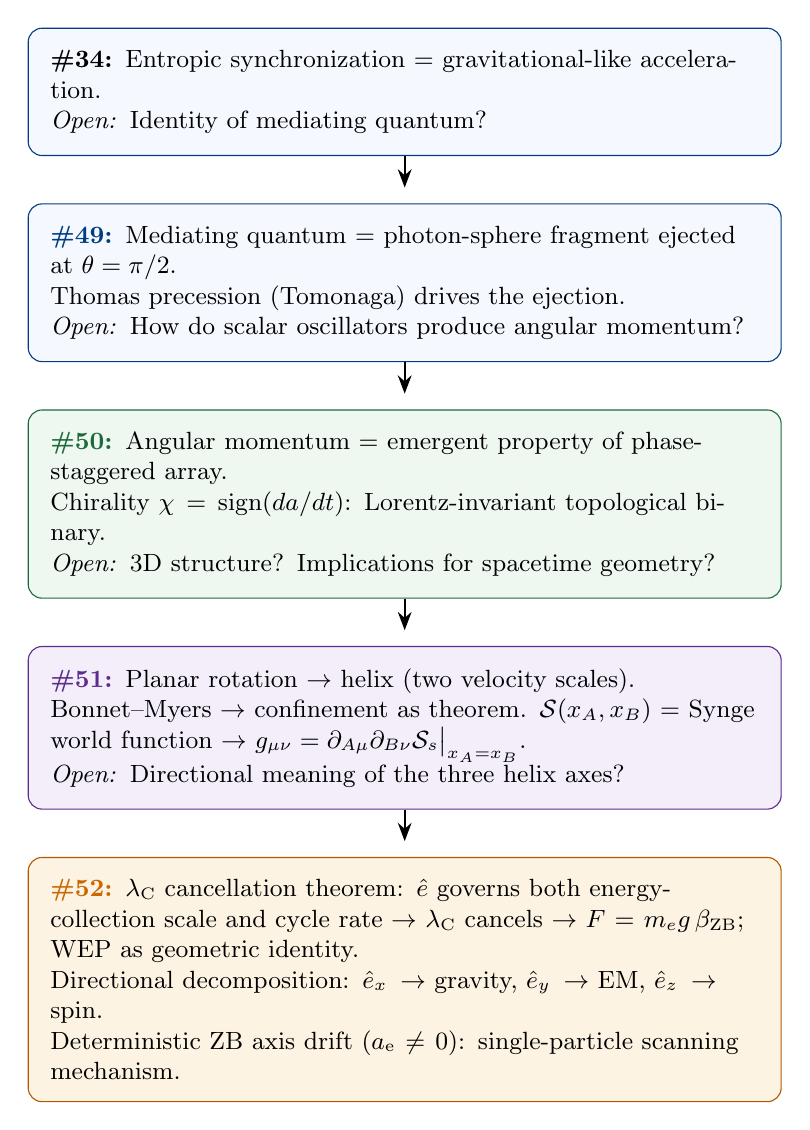
\begin{tikzpicture}[
  every node/.style={font=\small},
  box/.style={rectangle, rounded corners=5pt, draw, inner sep=8pt,
              text width=9cm, align=left},
  arr/.style={-Stealth, thick},
  qbox/.style={rectangle, draw=threadred!60, fill=warningbg,
               rounded corners=3pt, inner sep=6pt, text width=9cm,
               align=left, font=\small\itshape}
]
\node[box, fill=boxbg, draw=threadblue] (p34) at (0,0)
  {\textbf{\#34:} Entropic synchronization = gravitational-like acceleration.\\
   \textit{Open:} Identity of mediating quantum?};
\node[arr] at (0,-1.0) {};
\draw[arr] (p34.south) -- ++(0,-0.4) node[midway,right,font=\footnotesize]{};
\node[box, fill=boxbg, draw=threadblue, below=0.6cm of p34] (p49)
  {\textbf{\textcolor{threadblue}{\#49:}} Mediating quantum = photon-sphere fragment ejected at $\theta=\pi/2$.\\
   Thomas precession (Tomonaga) drives the ejection.\\
   \textit{Open:} How do scalar oscillators produce angular momentum?};
\draw[arr] (p49.south) -- ++(0,-0.4);
\node[box, fill=greenbg, draw=threadgreen, below=0.6cm of p49] (p50)
  {\textbf{\textcolor{threadgreen}{\#50:}} Angular momentum = emergent property of phase-staggered array.\\
   Chirality $\chi = \mathrm{sign}(da/dt)$: Lorentz-invariant topological binary.\\
   \textit{Open:} 3D structure? Implications for spacetime geometry?};
\draw[arr] (p50.south) -- ++(0,-0.4);
\node[box, fill=purplebg, draw=threadpurple, below=0.6cm of p50] (p51)
  {\textbf{\textcolor{threadpurple}{\#51:}} Planar rotation $\to$ helix (two velocity scales).\\
   Bonnet--Myers $\to$ confinement as theorem.
   $\calS(x_A,x_B)$ = Synge world function $\to$
   $g_{\mu\nu} = \partial_{A\mu}\partial_{B\nu}\calS_s\big|_{x_A=x_B}$.\\
   \textit{Open:} Directional meaning of the three helix axes?};
\draw[arr] (p51.south) -- ++(0,-0.4);
\node[box, fill=orangebg, draw=orange!70!black, below=0.6cm of p51] (p52)
  {\textbf{\textcolor{orange!80!black}{\#52:}} $\lambdaC$ cancellation theorem: $\hat{e}$ governs both energy-collection scale and cycle rate $\to$ $\lambdaC$ cancels $\to$ $F = m_eg\,\betaZB$; WEP as geometric identity.\\
   Directional decomposition: $\ehat{x}\to$ gravity, $\ehat{y}\to$ EM, $\ehat{z}\to$ spin.\\
   Deterministic ZB axis drift ($\anom\neq 0$): single-particle scanning mechanism.};
\end{tikzpicture}
\caption{The question chain across Papers \#34, \#49, \#50, \#51, and \#52.
Each paper closes one open question and opens the next.}
\label{fig:chain}
\end{figure}

\clearpage

% ============================================================
\section{Background Mathematics: A Textbook Introduction}
\label{sec:background}
% ============================================================

This section provides self-contained introductions to three mathematical tools
that are essential for the trilogy but may not be familiar to all readers.
The exposition is accessible to graduate students with knowledge of classical mechanics
and elementary differential geometry.

% ------------------------------------------------------------
\subsection{Thomas Precession: What It Is and Why It Matters}
\label{subsec:thomas}
% ------------------------------------------------------------

\subsubsection{The classical picture and its limitation}

The conventional picture of electron spin --- a spinning top precessing around a magnetic
field axis --- relies on the assumption that the electron moves in \emph{uniform circular
motion} with constant acceleration $\mathbf{a} = f$ (constant force).
Under this assumption, Thomas's formula
\begin{equation}
\boldsymbol{\Omega} = \frac{1}{2c^2}[\mathbf{a}\times\mathbf{v}]
\label{eq:thomas_general}
\end{equation}
yields a constant angular velocity, giving the precessing-top picture.
The $g$-factor of 2 appears as a factor-of-2 surprise: the naive classical calculation
gives $g=1$, and Thomas precession exactly doubles it.

\subsubsection{Thomas precession: Tomonaga's pedagogical account}

In his lecture book \textit{The Story of Spin}~\cite{Tomonaga1997}, written
for students, Tomonaga provides one of the clearest physical explanations of
\emph{why} Thomas precession is a kinematic inevitability --- not a dynamical
mechanism, but a geometric consequence of relativistic accelerated motion.
The essential point he conveys is this:

\begin{mdframed}[style=bluebox]
\textbf{Tomonaga's explanation (to students).}
For a body in uniform motion, the rest frame is unambiguously given by a Lorentz
transformation from the lab frame.  For a body in \emph{accelerated} motion,
even if we define the ``proper coordinate frame'' by requiring that its axes are
transported ``in parallel'' (each instant parallel to the infinitesimally preceding
instant), those axes, as seen from the lab, are \emph{not} in parallel transport
--- they rotate.
This rotation is not a consequence of the spatial path being curved.
It is a \emph{kinematic inevitability} of relativistic accelerated motion.
\end{mdframed}

In Tomonaga's own words (translated from~\cite{Tomonaga1997}, pp.~42--43):

\begin{quote}
``Thomas found that when the electron has an acceleration, the axis of the
coordinate system translating with the electron --- when viewed from the laboratory ---
does not move in parallel but is accompanied by a `rotation.' He found, through a
laborious calculation, that the axes of the proper coordinate system, as seen from
the laboratory, rotate with angular velocity
$\Omega = \frac{1}{2c^2}[\mathbf{a}\times\mathbf{v}]$.''
\end{quote}

This passage is Tomonaga \emph{explaining Thomas's result} to a student audience.
The angular velocity $\boldsymbol{\Omega}_T$ is non-zero whenever
$\mathbf{v}\times\mathbf{a}\neq\mathbf{0}$, i.e., whenever the acceleration has
a component perpendicular to the velocity.

\subsubsection{\texorpdfstring{Why a pendulum gives $\boldsymbol{\Omega}_T = \mathbf{0}$}{Why a pendulum gives Omega\_T = 0}}

For a pure one-dimensional oscillator (e.g., a pendulum or a spring along a fixed axis):
\begin{equation}
\mathbf{v}(t) = v_0\cos(\omega t)\,\hat{e}_x, \qquad
\mathbf{a}(t) = -v_0\omega\sin(\omega t)\,\hat{e}_x.
\end{equation}
Since $\mathbf{v}$ and $\mathbf{a}$ always point along the same axis,
$\mathbf{v}\times\mathbf{a} = \mathbf{0}$, and Thomas precession is absent.
The 0-Sphere model is categorically different.

\subsubsection{\texorpdfstring{The 0-Sphere case: SHM substitution (Paper \#10)}{The 0-Sphere case: SHM substitution (Paper \#10)}}

Paper~\paperno{10} \cite{hanamura10} was the first in the series to replace
the uniform-circular-motion assumption with SHM.
Setting $v = \cos\omega t$ and $a = -\sin\omega t$ and substituting into
Eq.~\eqref{eq:thomas_general}:
\begin{align}
\boldsymbol{\Omega}_T
&= \frac{1}{2c^2}[(-\sin\omega t)\times(\cos\omega t)] \notag\\
&= -\frac{1}{4c^2}\sin(2\omega t)\,\hat{e}_z.
\label{eq:omega_10}
\end{align}
The double angle $\sin(2\omega t)$ appears naturally, giving a period of $\pi$
rather than $2\pi$.
This is the first derivation in the series of the factor-of-2 (the $g=2$ structure)
from a kinematic argument.

\textit{However, Paper~\paperno{10} treated $v$ and $a$ as scalars without specifying
spatial directions.} Why are $\mathbf{v}$ and $\mathbf{a}$ perpendicular in the
0-Sphere model? This question was not answered until Papers~\paperno{49} and~\paperno{51}.

\subsubsection{\texorpdfstring{The answer: arc-curvature of the thermal geodesic (Papers \#49, \#51)}{The answer: arc-curvature of the thermal geodesic (Papers \#49, \#51)}}

The A$\to$B thermal geodesic is not a straight line but an arc-connected path in
three-dimensional space. Its curvature is what makes $\mathbf{v}\perp\mathbf{a}$:
\begin{align}
\mathbf{v}(t) &= v_0\cos(\omega t)\,\hat{e}_x \quad \text{(tangential to arc)},\\
\mathbf{a}(t) &= -v_0\omega\sin(\omega t)\,\hat{e}_y \quad \text{(transverse, curvature direction)},\\
\mathbf{v}\times\mathbf{a}
&= -\frac{v_0^2\omega}{2}\sin(2\omega t)\,\hat{e}_z \;\neq\; \mathbf{0}.
\label{eq:cross_product}
\end{align}
Substituting into Eq.~\eqref{eq:thomas_general}:
\begin{equation}
\boxed{\boldsymbol{\Omega}_T(\theta) = -\frac{v_0^2\omega}{4c^2}\sin(2\theta)\,\hat{e}_z, \qquad \theta = \omega t.}
\label{eq:omega_T}
\end{equation}
Because $\vZB\approx 0.04c$, the prefactor $v_0^2/c^2\approx 1.6\times10^{-3}$ is
small but non-negligible.
A purely Newtonian oscillator ($\vZB\to 0$) would give $\boldsymbol{\Omega}_T = \mathbf{0}$:
\emph{Thomas precession is inherently relativistic.}

\begin{mdframed}[style=openbox]
\textbf{Open task (item viii of \paperno{49}):}
The arc-curvature result establishes that $\mathbf{v}\times\mathbf{a}\neq\mathbf{0}$
qualitatively, but the \emph{quantitative} mapping from the thermal geodesic geometry
to the outward mechanical stress (in physical units) is not yet complete.
This is the central open task inherited by subsequent work.
\end{mdframed}

% ------------------------------------------------------------
\subsection{Synge's World Function: A Textbook Introduction}
\label{subsec:synge}
% ------------------------------------------------------------

\subsubsection{What is Synge's world function?}

Synge's world function, introduced by J.~L.~Synge \cite{Synge1960},
is a two-point scalar function that \emph{encodes all geometric information
about the geodesic connecting two spacetime points.}
It is defined as half the squared geodesic distance:
\begin{equation}
\sigma(x_A, x_B) \;\equiv\; \frac{1}{2}\,d^2(x_A, x_B),
\label{eq:synge_def}
\end{equation}
where $d(x_A, x_B)$ is the length of the (unique, shortest) geodesic between
the two points.

\subsubsection{Why is it useful?}

The metric tensor $g_{\mu\nu}$ can be recovered from $\sigma$ by a simple operation:
\begin{equation}
\boxed{g_{\mu\nu}(x) \;=\; \partial_{A\mu}\,\partial_{B\nu}\,\sigma(x_A, x_B) \Big|_{x_A = x_B = x}.}
\label{eq:synge_metric}
\end{equation}
This is the \emph{Synge reconstruction theorem}.
It holds for any two-point function $\sigma$ satisfying:
\begin{enumerate}[label=(\roman*), leftmargin=3em]
  \item $\sigma(x, x) = 0$ (vanishes at coincidence),
  \item $\sigma(x_A, x_B) = \sigma(x_B, x_A)$ (or the appropriate symmetrization),
  \item the mixed second derivatives at coincidence form a non-degenerate symmetric matrix.
\end{enumerate}

\subsubsection{Conceptual picture}

Think of $\sigma$ as a ``GPS distance function'' for curved spacetime.
Knowing the distance between any two nearby events, and knowing how that distance
changes as the events move, is \emph{equivalent} to knowing the full metric tensor.
Equation~\eqref{eq:synge_metric} makes this equivalence precise.

\begin{mdframed}[style=bluebox]
\textbf{Key analogy for intuition.}
In flat Euclidean space with metric $\delta_{ij}$:
\[
\sigma(x_A, x_B) = \frac{1}{2}\sum_i (x_A^i - x_B^i)^2.
\]
Computing $\partial_{Ai}\partial_{Bj}\sigma = -\partial_i^A\partial_j^A\sigma\big|_{x_A=x_B}
= \delta_{ij}$ immediately recovers the flat metric.
The theorem works in exactly the same way in curved spacetime, but with the geodesic
distance replacing the straight-line distance.
\end{mdframed}

\subsubsection{Applications in physics}

Synge's world function is a standard tool in:
\begin{itemize}[leftmargin=2em]
  \item \textbf{QFT in curved spacetime:}
        The propagator (Green's function) for a scalar field can be expressed as a
        function of $\sigma(x, x')$. The short-distance behavior (Hadamard expansion)
        is controlled by $\sigma$.
  \item \textbf{Hawking radiation:}
        Tracking the local behavior of the metric near the horizon requires the
        precise two-point geometric information encoded in $\sigma$.
  \item \textbf{Post-Newtonian approximation:}
        Gravitational wave calculations expand $\sigma$ in powers of $v/c$,
        systematically capturing relativistic corrections.
  \item \textbf{Numerical relativity:}
        Geodesic deviation (tidal forces) is governed by the second derivatives
        of $\sigma$ away from coincidence.
\end{itemize}

% ------------------------------------------------------------
\subsection{The Bonnet--Myers Theorem: Curvature Implies Finiteness}
\label{subsec:bonnet}
% ------------------------------------------------------------

\subsubsection{Statement of the theorem}

\begin{theorem}[Bonnet--Myers]
Let $(M, g)$ be a complete Riemannian manifold of dimension $n \geq 2$.
If the Ricci curvature satisfies $\mathrm{Ric}(v,v) \geq (n-1)K$ for all unit
vectors $v$, with $K > 0$, then:
\begin{equation}
\mathrm{diam}(M) \;\leq\; \frac{\pi}{\sqrt{K}}.
\end{equation}
In particular, $M$ is compact and has finite diameter.
\end{theorem}

\subsubsection{Physical meaning}

Positive Ricci curvature means that geodesics tend to converge (focus) rather than
diverge. The Bonnet--Myers theorem says that if this focusing is strong enough
(quantified by $K > 0$), the manifold cannot extend to infinite size: it must
be bounded.

For a sphere $S^n$ of radius $r$, the sectional curvature is $1/r^2$, so
$K = 1/r^2$ and $\mathrm{diam}(S^n) \leq \pi r$ --- which is the known exact result
(the diameter of a sphere equals $\pi r$, the length of a great semicircle).

\subsubsection{\texorpdfstring{Application to the 0-Sphere model (Paper \#51)}{Application to the 0-Sphere model (Paper \#51)}}

The photon sphere is modeled as $S^n$ ($n\geq 1$) with Compton-scale radius
$r\sim\lambdaC = \hbar/(m_e c) \approx 2.4\times10^{-12}$ m.
Applying Bonnet--Myers:
\begin{equation}
\mathrm{diam}(S^n_{\lambdaC}) \;\leq\; \pi r \;\sim\; \pi\lambdaC.
\label{eq:bonnet_bound}
\end{equation}
This bound is the geometric origin of the confinement domain $\mathcal{D}$ introduced
as an external assumption in Paper~\paperno{33}.
Paper~\paperno{51} \emph{derives} this confinement from the curvature of the photon
sphere, converting a topological input into a geometric theorem.

% ------------------------------------------------------------
\subsection{What the Line-Integral Programme Is Not: Three Common Misreadings}
\label{subsec:misreadings}
% ------------------------------------------------------------

A reader trained in standard quantum field theory or general relativity will
encounter the 0-Sphere line-integral programme with a set of pre-existing
conceptual templates.
Three of these templates naturally suggest themselves---and all three
lead to misreadings of the programme's actual mechanism.
Recording these misreadings explicitly serves a pedagogical purpose:
it prevents the reader from assimilating the new framework into a familiar
one that it superficially resembles but fundamentally is not.

\subsubsection{Misreading 1: coarse-graining (effective field theory)}

The standard approach to connecting microscopic and macroscopic physics
is the Wilsonian effective field theory (EFT) programme:
integrate out the fast (high-energy) degrees of freedom to obtain an effective
Lagrangian for the slow (low-energy) degrees of freedom.
The resulting effective theory has fewer degrees of freedom
and describes physics at longer length scales; the integrated-out information
is irretrievably lost.

The 0-Sphere programme contains a superficially similar hierarchy---a
fast internal cycle (Zitterbewegung at $\nu_{\mathrm{ZB}}\approx 5\times10^{18}$ Hz)
and slow external phenomena (gravitational coupling, electromagnetic radiation)---and
a reader may conclude that the external physics is obtained by ``averaging out''
or ``integrating out'' the fast internal dynamics.

\emph{This is not the mechanism.}
The phase accumulation functional $\calS(x_A,x_B) = \int_{\Gamma_{\mathrm{ext}}}\calA_\mu\,dx^\mu$
retains the complete internal history: no degrees of freedom are integrated out,
and no information is discarded.
The two force types are obtained not by a scale separation but by
\emph{two different differential operations on the same object}:
\begin{equation}
\underbrace{\int\!\mathcal{D}\phi_{\mathrm{heavy}}\;e^{iS[\phi_{\mathrm{light}},\phi_{\mathrm{heavy}}]}}_{\text{EFT: integrate out (information lost)}}
\quad\neq\quad
\underbrace{\calS(x_A,x_B)
\;\xrightarrow[\text{endpoint variation}]{\text{path deformation}}\;
\begin{cases}
\mathcal{F}_{\mu\nu}\\[2pt]
g_{\mu\nu}
\end{cases}}_{\text{0-Sphere: directional bifurcation (information retained)}}
\label{eq:eft_vs_0sm}
\end{equation}
The left-hand side produces one effective theory at the cost of losing
microscopic detail; the right-hand side produces two physical sectors
while preserving the full content of the phase history.
This distinction is not a matter of taste but of mathematical structure:
EFT requires a scale hierarchy ($\Lambda_{\mathrm{UV}}\gg\Lambda_{\mathrm{IR}}$);
the 0-Sphere bifurcation operates at a single scale ($\sim\lambdaC$).

\subsubsection{Misreading 2: statistical averaging}

Paper~\paperno{52} derives $F = m_e g\,(\vZB/c)$ (with $\vZB/c\approx 0.04$ a
free-parameter-free prediction from the anomalous magnetic moment) for a single electron
in a gravitational field, with the force arising from the deterministic drift of the ZB axis
$\hat{e}$ and the asymmetric ejection probability at turning points.
A natural reading is that this derivation involves a statistical average
over many ZB cycles, analogous to the way thermodynamic quantities
emerge from ensemble averages in statistical mechanics.

\emph{This is not the mechanism.}
The 0-Sphere derivation is explicitly \emph{Lagrangian} (single-particle):
the electron has a definite internal state $(\iphase(t), \hat{e}(t))$ at
each instant, and the gravitational force is the actual momentum transferred
per cycle to this specific particle, not the expectation value of a force
operator applied to an ensemble~\cite{hanamura52}.

The angular momentum conservation established in Paper~\paperno{50}
provides a parallel illustration.
The net torque from the radiation gradient $F(\iphase)=E_0\sin\iphase$
averages to zero over one cycle---but this vanishing is not a statistical
cancellation; it is an exact algebraic identity
$\sum_k\sin(b_k - a) = 0$ that holds for every value of $a$
under the uniform angular distribution of oscillator axes~\cite{hanamura50}.
The angular momentum is a \emph{topologically protected constant of motion}
on $S^1$, not a statistical average over fluctuating microstates.

The probabilistic character that standard quantum mechanics assigns to
$F = mg$ is, in the 0-Sphere framework, \emph{epistemic}:
it reflects the external observer's ignorance of the hidden variables
$(\iphase, \hat{e})$, not any fundamental randomness in the dynamics.
This is Einstein's realist programme carried through at the mechanical level.

\subsubsection{Misreading 3: derivative-order hierarchy as scale separation}

Paper~\paperno{40} identified a structural asymmetry between gauge theory
(force at the curvature level, $F_{\mu\nu}$: second derivative of the potential)
and general relativity (force at the connection level, $\Gamma^\mu_{\nu\rho}$:
first derivative of the metric).
A reader familiar with effective field theory may interpret this as a
renormalization-group hierarchy: the first-derivative (connection) description
is the ``IR'' effective theory, and the second-derivative (curvature)
description is the ``UV'' completion.

\emph{This is not the mechanism.}
In the 0-Sphere programme, the two derivative orders arise from
two projections of a single functional $\calS$ at the \emph{same} scale
(the Compton scale $\lambdaC$).
Paper~\paperno{51} proposes the resolution explicitly~\cite{hanamura51}:
\begin{itemize}[leftmargin=2em, itemsep=4pt]
  \item \textbf{Path deformation} of $\calS$
        $\;\longrightarrow\;$ Berry curvature $\mathcal{F}_{\mu\nu}$
        (gauge sector; second-derivative structure).
  \item \textbf{Endpoint variation} of $\calS$
        $\;\longrightarrow\;$ metric $g_{\mu\nu}$
        (gravitational sector; the connection $\Gamma^\mu_{\nu\rho}$
        descends from $g_{\mu\nu}$ by one further derivative).
\end{itemize}
Paper~\paperno{52} provides the directional counterpart of this algebraic
bifurcation~\cite{hanamura52}: the $\ehat{y}$ direction (transverse oscillation)
corresponds to path deformation and the electromagnetic sector,
while the $\ehat{x}$ direction (longitudinal propagation) corresponds to
endpoint variation and the gravitational sector.

The apparent ``hierarchy'' between 1st and 2nd derivative orders is
therefore not a scale hierarchy but a \emph{directional} one:
the same phase-history object $\calS$, differentiated in two orthogonal
directions of the helical geometry, produces objects of different
derivative order.
There is no UV/IR separation, no running coupling, and no
renormalization-group flow involved.

\begin{mdframed}[style=chainbox]
\textbf{Summary of the three misreadings.}
\renewcommand{\arraystretch}{1.3}
\begin{tabular}{p{3.0cm}p{4.5cm}p{5.0cm}}
\toprule
\textbf{Misreading} & \textbf{Familiar template} & \textbf{Actual 0-Sphere mechanism} \\
\midrule
Coarse-graining &
  EFT: integrate out fast DOF &
  Directional bifurcation of $\calS$; no DOF lost \\
\addlinespace[0.15cm]
Statistical averaging &
  Ensemble average $\to$ macroscopic force &
  Single-particle deterministic drift; topological protection \\
\addlinespace[0.15cm]
Scale separation &
  UV/IR hierarchy; RG flow &
  Same scale ($\lambdaC$); directional, not hierarchical \\
\bottomrule
\end{tabular}
\end{mdframed}

\noindent The common thread across all three misreadings is the assumption
that the internal and external descriptions belong to \emph{different scales}
that are connected by an averaging or coarsening operation.
The 0-Sphere programme replaces this vertical (scale) separation with
a horizontal (directional) one:
internal and external physics coexist at the same Compton scale,
and the distinction between gauge forces and gravity is encoded in
the direction---not the magnitude---of differentiation of the phase history.

\clearpage

% ============================================================
\section{\texorpdfstring{Paper \#49 in Detail: The Ejection Mechanism}{Paper \#49 in Detail: The Ejection Mechanism}}
\label{sec:p49}
% ============================================================

\begin{mdframed}[style=bluebox]
\textbf{\textcolor{threadblue}{Paper \#49:}}
``Photon-Sphere Fragmentation as a Gravitational Mediator:
Radiation-Gradient Ejection in the $\pi$-Cycle of the 0-Sphere Model''\\
DOI: \doilink{10.5281/zenodo.19393391} $|$ April 4, 2026 $|$ \textit{Essential}
\end{mdframed}

% ------------------------------------------------------------
\subsection{\texorpdfstring{The $\pi$-Cycle and the Ejection Threshold}{The pi-Cycle and the Ejection Threshold}}
\label{subsec:pi_cycle}
% ------------------------------------------------------------

The photon sphere oscillates between Kernel~A ($\theta = 0$) and Kernel~B
($\theta = \pi$) under the radiation gradient
\begin{equation}
F(\theta) \;=\; \frac{d}{d\theta}(Te_2 - Te_1) \;=\; E_0\sin\theta.
\label{eq:radiation_gradient}
\end{equation}
The photon-sphere kinetic energy profile over the $\pi$-cycle is:
\begin{equation}
E_{\mathrm{ph}}(\theta) \;=\; \frac{E_0}{2}\sin^2\theta.
\label{eq:eph_profile}
\end{equation}
This peaks at $\theta = \pi/2$ (the midpoint of the traversal) with value
$E_{\mathrm{ph}}(\pi/2) = E_0/2$.

The zero-point energy floor of the Hamiltonian --- established in Paper~\paperno{46}
via the AM--GM inequality and confirmed three independent ways in Paper~\paperno{48}
--- is also $E_0/2$.

\begin{mdframed}[style=bluebox]
\textbf{Ejection threshold:}
\begin{equation}
E_{\mathrm{ph}}(\pi/2) \;=\; E_0/2 \;=\; E_{\mathrm{bind}}.
\label{eq:threshold}
\end{equation}
\begin{itemize}[leftmargin=1.5em, itemsep=2pt]
  \item $n = 0$ (ground state): threshold exactly saturated; no surplus energy;
        photon-sphere fragment is \emph{not} ejected.
  \item $n \geq 1$ (excited state): surplus $n\hbar\omega$ above the floor is available;
        one quantum $\hbar\omega$ is ejected per de-excitation $n\to n-1$.
\end{itemize}
\end{mdframed}

\noindent The physical picture: each excited state $n$ carries $n+1$ antinodes in its
standing-wave profile, providing $n+1$ ejection opportunities per A$\to$B traversal.

\subsection{Thomas-Precession Ejection: Conceptual Revision in Paper \#49}
\label{subsec:tomonaga}

The critical conceptual revision of Paper~\paperno{49} is the replacement of the
``arc-curvature'' framing of Thomas precession (used implicitly in earlier papers)
with a framing that places the physical cause correctly at the level of relativistic
accelerated motion itself --- a kinematic inevitability of special relativity that
Thomas identified in 1927 and that Tomonaga explained with particular clarity
for students in \textit{The Story of Spin} \cite{Tomonaga1997}.
Table~\ref{tab:framing} summarizes the change.

\begin{table}[h!]
\centering
\renewcommand{\arraystretch}{1.4}
\begin{tabular}{p{3.5cm}p{5.0cm}p{5.0cm}}
\toprule
 & \textbf{Old framing} & \textbf{New framing (\#49)} \\
\midrule
\textbf{Cause} & Arc-connected path $\to$ curvature $\to$ $\mathbf{v}\times\mathbf{a}\neq\mathbf{0}$ &
  Relativistic accelerated motion $\to$ kinematic inevitability (Thomas 1927; clearly explained by Tomonaga \cite{Tomonaga1997}) \\
\addlinespace[0.2cm]
\textbf{Primary driver} & Geometric path curvature &
  Radiation gradient $F(\theta)=E_0\sin\theta$ \\
\addlinespace[0.2cm]
\textbf{$\mathbf{v}\times\mathbf{a}\neq\mathbf{0}$} & Explanation &
  Concrete expression of the above \\
\addlinespace[0.2cm]
\textbf{Reference} & --- &
  Tomonaga, \textit{The Story of Spin} (1997) \cite{Tomonaga1997} \\
\bottomrule
\end{tabular}
\caption{Conceptual revision of the Thomas precession framing in Paper~\paperno{49}.
See also \texttt{tomonaga.md} in the repository for the full anti-pattern and cross-reference list.}
\label{tab:framing}
\end{table}

\noindent The Thomas angular velocity at the ejection point $\theta=\pi/2$ is:
\begin{equation}
\OmT\!\left(\frac{\pi}{2}\right)
\;=\; -\frac{v_0^2\omega}{4c^2}\sin(\pi)\,\hat{e}_z \;=\; 0_{\text{(extremum)}},
\end{equation}
but the \emph{magnitude} $|\OmT(\theta)|$ peaks near $\theta=\pi/4$ and $3\pi/4$,
generating outward centrifugal-like stress throughout the traversal that reaches its
cumulative maximum effect at $\theta=\pi/2$.

\subsection{\texorpdfstring{Four Independent Routes to $E_0/2$}{Four Independent Routes to E_0/2}}

Paper~\paperno{49} establishes the \emph{fourth independent route} to the zero-point energy $\frac{1}{2}\hbar\omega$, completing what Paper~\paperno{48} named the ``triple coincidence.'' Table~\ref{tab:four_routes} collects all four routes and their mathematical origins.

\begin{table}[h!]
\centering
\renewcommand{\arraystretch}{1.4}
\begin{tabular}{p{1cm}p{3.5cm}p{5.5cm}p{2.5cm}}
\toprule
\textbf{\#} & \textbf{Route} & \textbf{Mathematical origin} & \textbf{Paper} \\
\midrule
1 & QM uncertainty principle &
  $[\hat{x}, \hat{p}] = i\hbar \;\Rightarrow\; \Delta x\cdot\Delta p \geq \hbar/2$ &
  Standard QM \\
\addlinespace[0.2cm]
2 & Hamiltonian identity (AM--GM) &
  $\cos^4(\theta/2)+\sin^4(\theta/2) \geq \frac{1}{2}$ (algebraic) &
  \paperno{46} \\
\addlinespace[0.2cm]
3 & Centroid geometry &
  AM--GM on $(\cos^2\theta, \sin^2\theta)$ $\Rightarrow$ centroid radius $\geq 1/2$ &
  \paperno{48} \\
\addlinespace[0.2cm]
4 & Ejection threshold &
  $E_{\mathrm{ph}}(\pi/2) = E_0/2 = E_{\mathrm{bind}}$ (physical) &
  \paperno{49} (\textit{new}) \\
\bottomrule
\end{tabular}
\caption{Four independent routes to the zero-point energy floor $E_0/2$.
All four arise from the single algebraic constraint $\cos^2\theta + \sin^2\theta = 1$.}
\label{tab:four_routes}
\end{table}

\subsection{Structural Ultraviolet Cutoff}

Re-absorption of an ejected fragment by the same electron constitutes the 0-Sphere
counterpart of a QED self-energy loop. The key observation is that mode $n$ has $n+1$
antinodes, and therefore $n+1$ re-absorption opportunities per A$\to$B traversal.
Because $n$ is bounded above by $n_{\max}$ (set by the Compton-scale geometry of the
Kernel~A--B potential well), the self-energy sum is finite without regularization:
\begin{equation}
\Sigma_{\text{self}} \;=\; \sum_{n=0}^{n_{\max}} w_n \;\cdot\; (n+1)\hbar\omega
\;\;<\;\; \infty.
\end{equation}
This is a \emph{Debye-type structural cutoff}: the finite size of the internal structure
replaces the ad hoc regularization required in standard QED.

\begin{mdframed}[style=openbox]
\textbf{Open task (item ix of \paperno{49}):}
The existence of $n_{\max}$ is established; its quantitative value requires a derivation
of $\vZB(n)$ (the ZB velocity as a function of excitation number).
\end{mdframed}

\clearpage

% ============================================================
\section{\texorpdfstring{Paper \#50 in Detail: From Scalar Oscillations to Angular Momentum}{Paper \#50 in Detail: From Scalar Oscillations to Angular Momentum}}
\label{sec:p50}
% ============================================================

\begin{mdframed}[style=greenbox]
\textbf{\textcolor{threadgreen}{Paper \#50:}}
``Rotation from Scalar Oscillation: Emergence of Angular Momentum, Chirality, and Helicity
in the 0-Sphere Model'' $|$ \doilink{10.5281/zenodo.19482145} $|$ \textit{Essential}
\end{mdframed}

\subsection{The Apparent Paradox}

The kernel energies $Te_1 = E_0\cos^4(\theta/2)$ and $Te_2 = E_0\sin^4(\theta/2)$
are scalar potentials in the internal phase $\theta$. A scalar potential has no preferred
rotation direction; its gradient is purely radial. How can such a system generate
angular momentum $L_z = \hbar$?

\subsection{Phase-Staggered Oscillator Array}

Consider $n$ radial oscillation axes, uniformly distributed in angle, with amplitude
\begin{equation}
P_k(a) = \cos(a - b_k), \qquad b_k = \frac{k\pi}{n}, \quad k=0,1,\ldots,n-1.
\end{equation}
Each oscillator moves strictly along its own radial axis. Nevertheless, as the global
phase $a$ increases continuously, the \emph{locus of maximum amplitude} sweeps around
the unit circle --- an emergent rotation from purely linear constituents.

\textbf{Centroid locus.} The centroid of all $n$ oscillators (exact in the continuum limit):
\begin{equation}
\bar{x}(a) \to \frac{\cos a}{2}, \qquad \bar{y}(a) \to \frac{\sin a}{2}.
\end{equation}
The centroid traces a circle of radius \emph{exactly} $\frac{1}{2}$, independently of $n$.

\begin{mdframed}[style=greenbox]
\textbf{Key connection.}
The centroid radius $\frac{1}{2}$ and the energy floor $E_0/2$ are \emph{two projections
of the same AM--GM constraint:}
\begin{equation}
\cos^2\iphase + \sin^2\iphase = 1
\;\;\Rightarrow\;\;
\frac{\cos^2\iphase + \sin^2\iphase}{2} \geq \sqrt{\cos^2\iphase\cdot\sin^2\iphase}
\;\;\Rightarrow\;\;
\frac{1}{2} \geq |\cos\iphase\sin\iphase|.
\end{equation}
Both the spatial support (centroid cannot reach the origin) and the energy (photon-sphere
energy bounded above by $E_0/2$) are consequences of this single algebraic inequality.
\end{mdframed}

\subsection{Thomas Precession as a Relativistic Window}

The role of Thomas precession in the 0-Sphere framework was fundamentally revised
in Paper~\paperno{50}:

\begin{mdframed}[style=greenbox]
\begin{center}
\textbf{Old picture (implicit in \paperno{10}--\paperno{49}):}\par\vspace{4pt}
Thomas precession \emph{generates} angular momentum.
\end{center}

\vspace{0.3cm}
\begin{center}
\textbf{New picture (\paperno{50}):}\par\vspace{4pt}
Angular momentum exists as a \emph{topological invariant} of the $S^1$ phase flow,
independently of any relativistic correction.
Thomas precession is the \emph{relativistic window} through which this topologically
existing angular momentum becomes observable in the lab.
\end{center}
\end{mdframed}

\noindent Specifically (Paper~\paperno{50}, Section~7.1, item~4):
\begin{quotation}\noindent
``Thomas precession provides the relativistic geometric correction through which the
phase-space rotation becomes observable in the laboratory frame.
It does not generate the circular structure --- that structure exists at the topological
level of the $S^1$ phase flow independently of any relativistic correction ---
but it quantifies the physical scale of the phase stagger $\delta b = \pi/n$
in terms of $\vZB$, and accounts for the accumulation of $a_e$ per internal cycle.''
\end{quotation}

\noindent In the Newtonian limit $\vZB/c\to 0$:
the $S^1$ phase flow, chirality $\chi$, and $4\pi$ periodicity all survive,
but $\OmT\to\mathbf{0}$, $a_e\to 0$,
and the phase stagger becomes externally unmeasurable.

\subsection{Chirality: Lorentz-Invariant Topological Binary}

\begin{equation}
\boxed{\chi \;\equiv\; \mathrm{sign}(da/dt)}
\end{equation}
where $\chi$ is the orientation of the phase flow on $S^1$, i.e., the sign of the winding number of the directed geodesic.

$\chi$ is classified by $\pi_1(S^1) = \mathbb{Z}$; its sign is Lorentz invariant
because Lorentz boosts preserve the orientation of directed curves.
Table~\ref{tab:chirality} compares the QFT vocabulary for chirality and helicity with the corresponding 0-Sphere geometric objects.

\begin{table}[h!]
\centering
\renewcommand{\arraystretch}{1.4}
\begin{tabular}{p{3.2cm}p{4.3cm}p{5.5cm}}
\toprule
\textbf{Concept} & \textbf{QFT standard} & \textbf{0-Sphere Model} \\
\midrule
Chirality $\chi$ & $\gamma^5$ eigenvalue $(\pm 1)$ &
  $\mathrm{sign}(da/dt)$: winding sign on $S^1$ \\
Right-chiral ($\psi_R$) & Upper Weyl spinor &
  Forward geodesic; Kernel~A dominant \\
Left-chiral ($\psi_L$) & Lower Weyl spinor &
  Backward geodesic; Kernel~B dominant \\
Helicity $h$ & $\mathbf{S}\cdot\hat{\mathbf{p}}/|\mathbf{p}|$ &
  Rotation direction in $yz$-plane from $-x$ \\
Lorentz invariance & $\chi$: yes; $h$: no &
  Geodesic orientation ($S^1$ winding): yes \\
Helicity flip & $v_{\mathrm{obs}} > v_{\mathrm{particle}}$ &
  CCW $\to$ CW as seen by overtaking observer \\
Mass--helicity link & Flip forbidden at $m=0$ &
  $\vZB\to 0$ as $m\to 0$: no rotation, no flip \\
\bottomrule
\end{tabular}
\caption{Chirality and helicity: QFT standard vs.\ 0-Sphere Model vocabulary.}
\label{tab:chirality}
\end{table}

\subsection{\texorpdfstring{The Three Faces of $\frac{1}{2}$: Answering \#47's Open Question}{The Three Faces of 1/2: Answering \#47's Open Question}}

Paper~\paperno{47} identified three independent occurrences of the factor $\frac{1}{2}$
in the 0-Sphere framework and predicted that their common geometric origin would be
examined in a future paper. Paper~\paperno{50} provides that answer, tracing all three back to the algebraic constraint $\cos^2\theta + \sin^2\theta = 1$ under the AM--GM inequality; the correspondence is displayed in Table~\ref{tab:threehalf}.

\begin{table}[h!]
\centering
\renewcommand{\arraystretch}{1.4}
\begin{tabular}{p{1.5cm}p{3.5cm}p{5.5cm}p{1.5cm}}
\toprule
\textbf{Face} & \textbf{Type} & \textbf{Statement} & \textbf{Paper} \\
\midrule
Centroid radius &
  \textit{Geometric} &
  Phase-staggered array centroid: radius $= \frac{1}{2}$, independent of $n$ &
  \paperno{50} \\
\addlinespace[0.2cm]
Thomas coefficient &
  \textit{Kinematic} &
  $\OmT \approx \frac{1}{2}\frac{\mathbf{v}}{c^2}\times\mathbf{a}$;
  without this, hydrogen spin-orbit splitting doubles &
  \paperno{10, 50} \\
\addlinespace[0.2cm]
Spin quantum number &
  \textit{Topological} &
  $s = \frac{1}{2}$: spinor requires $4\pi$ rotation to return to original value &
  \paperno{26, 50} \\
\midrule
Common root & \textit{Algebraic} &
  All three reflect $\cos^2\theta + \sin^2\theta = 1$ under AM--GM &
  \paperno{50} \\
\bottomrule
\end{tabular}
\caption{The three faces of $\frac{1}{2}$ in the 0-Sphere Model,
and their common algebraic root (Paper~\paperno{50}, Section~7.4).}
\label{tab:threehalf}
\end{table}

\subsection{Four Dirac Components from Geometry}

\begin{equation}
\text{4 Dirac spinor components}
\;=\; \chi\in\{+1,-1\} \;\times\; \mathrm{spin}\in\{+\tfrac{1}{2},-\tfrac{1}{2}\}
\;=\; 2\times 2 \;=\; 4.
\end{equation}
The electron/positron distinction is carried by $\chi$ (direction of geodesic traversal).
The two spin states are carried by the up/down orientation of the angular momentum
generated by the phase-staggered array.
No additional quantum numbers are postulated.

\clearpage

% ============================================================
\section{\texorpdfstring{Paper \#51 in Detail: From Topology to the Spacetime Metric}{Paper \#51 in Detail: From Topology to the Spacetime Metric}}
\label{sec:p51}
% ============================================================

\begin{mdframed}[style=purplebox]
\textbf{\textcolor{threadpurple}{Paper \#51:}}
``Helical Trajectory, Fixed-Endpoint Line Integrals, and the Emergence of the
Spacetime Metric in the 0-Sphere Model'' $|$ \doilink{10.5281/zenodo.19489126} $|$ \textit{Essential}
\end{mdframed}

% ------------------------------------------------------------
\subsection{The Master Logical Chain}
\label{subsec:master_chain}
% ------------------------------------------------------------

Paper~\paperno{51} establishes an unbroken logical chain from a topological
observation about the 0-Sphere to a proposal for the emergence of the spacetime metric.
This chain is the central contribution of the paper and the culmination of the trilogy.

\begin{mdframed}[style=chainbox]
\begin{center}
\textbf{The Logical Chain of Paper \#51}
\end{center}

\vspace{0.3cm}
\textbf{Step 1. Topological input.}\\
$S^0 = \{A,B\}$ consists of exactly two isolated points.
Two isolated points are \emph{not arcwise connected}: no continuous curve can travel
from $A$ to $B$ while remaining in $S^0$.

\vspace{0.4cm}
$\downarrow$ \textit{arcwise-connected embedding required}

\vspace{0.4cm}
\textbf{Step 2. Embedding.}\\
The photon sphere, modeled as $S^n$ ($n\geq 1$), is arcwise connected and provides
the required embedding space. Each point in $S^0$ is identified with a point in $S^n$.

\vspace{0.4cm}
$\downarrow$ \textit{Compton-scale radius $r\sim\lambdaC$ + positive curvature}

\vspace{0.4cm}
\textbf{Step 3. Bonnet--Myers theorem (Theorem~\ref{thm:BM}).}\\
\begin{equation}
\mathrm{diam}(S^n_{\lambdaC}) \;\leq\; \pi r \;\sim\; \pi\lambdaC.
\tag{Bonnet--Myers}
\end{equation}
This finite diameter bound defines the confinement domain $\mathcal{D}$ of
Paper~\paperno{33} as a \emph{geometric theorem}, not an external assumption.

\vspace{0.4cm}
$\downarrow$ \textit{lower bound from two-point connectivity}

\vspace{0.4cm}
\textbf{Step 4. Separation bounds.}\\
\begin{equation}
0 \;<\; |x_A - x_B| \;\leq\; \pi\lambdaC.
\label{eq:separation_bounds}
\end{equation}
Both upper and lower bounds are derived from the two-kernel geometry.

\vspace{0.4cm}
$\downarrow$ \textit{non-antipodality of Kernels A and B}

\vspace{0.4cm}
\textbf{Step 5. Uniqueness of thermal geodesic.}\\
The kernel separation satisfies $|x_A - x_B|\sim\lambdaC/2 < \pi r = \mathrm{diam}(S^n)$,
so Kernels~A and~B are \emph{not antipodal}. By the geodesic uniqueness theorem for
non-antipodal pairs on compact Riemannian manifolds, the thermal geodesic connecting
$A$ to $B$ is \emph{unique}.

\vspace{0.4cm}
$\downarrow$ \textit{uniqueness $\Rightarrow$ well-defined two-point functional}

\vspace{0.4cm}
\textbf{Step 6. Phase accumulation functional.}\\
The Berry connection 1-form $\calA_\mu$ encodes the spinorial phase acquired during
transport along the helical arc. The phase accumulated along the \emph{unique} extremal
arc $\Gamma_{\mathrm{ext}}$ is:
\begin{equation}
\calS(x_A, x_B) \;\equiv\; \int_{\Gamma_{\mathrm{ext}}(x_A,x_B)} \calA_\mu\,dx^\mu.
\label{eq:S_def}
\end{equation}
Because the arc is unique, $\calS$ depends only on the endpoint pair $(x_A, x_B)$,
not on any choice of path.

\vspace{0.4cm}
$\downarrow$ \textit{three structural properties verified}

\vspace{0.4cm}
\textbf{Step 7. Identification with Synge's world function.}\\
$\calS(x_A, x_B)$ satisfies the three Synge axioms:
\begin{enumerate}[label=(\roman*), leftmargin=3em, itemsep=2pt]
  \item $\calS(x,x) = 0$ (coincidence: arc degenerates to a point),
  \item $\calS(x_B,x_A) = -\calS(x_A,x_B)$ (antisymmetry: reversed traversal),
  \item $\calS_s \equiv \frac{1}{2}[\calS(x_A,x_B)+\calS(x_B,x_A)]$
        has non-degenerate mixed second derivatives.
\end{enumerate}
Therefore $\calS_s$ may be identified with a generalized Synge world function:
\begin{equation}
\underbrace{\sigma(x_A,x_B)}_{\text{Synge}}
\;\longleftrightarrow\;
\underbrace{\calS_s(x_A,x_B)}_{\text{0-Sphere}}.
\label{eq:synge_identification}
\end{equation}

\vspace{0.4cm}
$\downarrow$ \textit{Synge reconstruction theorem applied}

\vspace{0.4cm}
\textbf{Step 8. Metric emergence proposal.}
\begin{equation}
\boxed{g_{\mu\nu}(x) \;=\; \partial_{A\mu}\,\partial_{B\nu}\,\calS_s(x_A, x_B) \Big|_{x_A = x_B = x}.}
\label{eq:metric_proposal}
\end{equation}
The spacetime metric emerges as the second functional derivative of the internal
phase history. The standard GR derivation proceeds
$g_{\mu\nu}\to\Gamma^\mu_{\nu\rho}\to R^\mu{}_{\nu\rho\sigma}$;
the present construction inverts the first step:
$\calA_\mu\to\calS\to g_{\mu\nu}$.
\end{mdframed}

\begin{theorem}[Bonnet--Myers applied to the photon sphere]
\label{thm:BM}
Let the photon sphere be modeled as $S^n$ $(n\geq 1)$ with radius
$r\sim\lambdaC$ and sectional curvature $K = 1/r^2 > 0$.
Then $\mathrm{diam}(S^n)\leq\pi r\sim\pi\lambdaC$,
and the confinement domain $\mathcal{D}$ of Paper~\paperno{33} is realized
as a geometric theorem.
\end{theorem}

\subsection{The Helical Trajectory and Two Velocity Scales}
\label{subsec:helix}

Paper~\paperno{50} established that the photon sphere rotates in the transverse ($yz$)
plane. Paper~\paperno{51} adds the longitudinal advance along the propagation ($x$) axis:
the active kernel shuttles between Kernel~A and Kernel~B separated by $\Delta x\sim\lambdaC$,
converting the planar circle into a three-dimensional helix.

The distinctive result is the identification of \emph{two separate velocity scales}, summarized in Table~\ref{tab:velocities}:

\begin{table}[h!]
\centering
\renewcommand{\arraystretch}{1.4}
\begin{tabular}{p{3.5cm}p{2.5cm}p{3.5cm}p{3.5cm}}
\toprule
\textbf{Scale} & \textbf{Value} & \textbf{Physical origin} & \textbf{Prediction} \\
\midrule
Transverse ($\vZB$) & $\approx 0.04c$ &
  AMM: $\gamma = 1 + a_e$ (Paper~\paperno{10}) &
  ZB frequency $\nu_{\mathrm{ZB}}\approx 5\times10^{18}$ Hz (X-ray) \\
\addlinespace[0.2cm]
Longitudinal ($v_{\mathrm{pitch}}$) & $\sim c$ &
  Compton separation $\Delta x\sim\lambdaC$ and $\omega_{\mathrm{ZB}}$ &
  Dirac $\pm c$ recovered as projection \\
\addlinespace[0.2cm]
Ratio & $\approx 25$ & Two-kernel architecture & Breaks Dirac--Hestenes uniformity \\
\bottomrule
\end{tabular}
\caption{Two velocity scales in the helical trajectory (Paper~\paperno{51}, Section~2).
The Dirac--Hestenes model assumes a uniform speed $c$; the 0-Sphere Model identifies
two physically distinct dynamical processes.
\emph{Important:} ``transverse'' and ``longitudinal'' here denote
dynamically distinct processes, not spatial wave components.}
\label{tab:velocities}
\end{table}

\noindent The ZB frequency predicted by the 0-Sphere Model:
\begin{equation}
\nu_{\mathrm{ZB}} = \frac{\vZB}{\lambdaC} \approx 5.0\times10^{18}\;\mathrm{Hz}
\quad (\text{X-ray regime}),
\end{equation}
compared to the Dirac prediction $\nu_{\mathrm{ZB}}^{\mathrm{Dirac}} = mc^2/(\pi\hbar)
\approx 3.93\times10^{20}$ Hz (gamma-ray regime).
The factor of $\sim 80$ difference arises from replacing $c$ by $\vZB\approx 0.04c$.

\subsubsection{Two-Scale Structure: Physical Interpretation and Terminological Caution}
\label{subsubsec:two_scale}

\begin{mdframed}[style=purplebox]
\textbf{Terminological caution.}
The labels ``transverse'' and ``longitudinal'' used throughout this section
do \emph{not} refer to transverse and longitudinal wave components in the usual
sense of wave mechanics (e.g., polarization directions of a photon).
They denote two \emph{dynamically independent processes}:
the transverse scale ($\vZB$) characterizes \emph{internal field transitions}
(the A--B emission-absorption cycle),
while the longitudinal scale ($v_{\mathrm{pitch}}$) characterizes
\emph{global relativistic propagation} along the worldline.
This distinction must be kept in mind to avoid misidentifying the model's
predictions with properties of spatial wave modes.
\end{mdframed}

The two dynamical processes are physically independent and arise from different origins:

\paragraph{Internal dynamics ($\vZB \approx 0.04c$).}
The internal scale arises from the cyclic radiation-and-absorption process between
Kernel~A and Kernel~B. This quantity does not represent the propagation speed of a
free particle or photon, but rather an effective rate characterizing the
internal energy-exchange cycle. Concretely, $\vZB$ is derived from the anomalous
magnetic moment via $\gamma = 1 + a_e$, without any appeal to kinematic decomposition
of a larger velocity. The internal dynamics take place along a \emph{thermal geodesic}
in the abstract internal field (configuration) space, not through physical space.
The effective velocity $\vZB$ therefore characterizes the rate of traversal along
this internal path.

\paragraph{Global propagation ($v_{\mathrm{pitch}} \sim c$).}
The longitudinal scale represents the cumulative drift along the helical axis generated
by successive internal transitions. More precisely, $v_{\mathrm{pitch}}$ is an effective
propagation velocity along the worldline. Since this propagation corresponds to a
relativistic trajectory, it saturates the relativistic upper bound, and the estimate
$v_{\mathrm{pitch}}\sim c$ should be understood as saturation of this limit, not as a
claim that an internal constituent moves at exactly $c$.

\paragraph{Composite helical motion and the Dirac result.}
The helical structure arises as a composite effect of these two scales. The A--B
transition cycle generates the rotational component; relativistic propagation produces
the axial drift. The resulting asymmetry, quantified by the ratio
$v_{\mathrm{pitch}}/\vZB \approx 25$, plays a central role in determining the
observed chirality.

In the Dirac theory, the velocity operator has eigenvalues $\pm c$ along any given axis.
In the present model, these luminal eigenvalues are not taken to imply that all
\emph{internal} dynamics occur at the speed of light. Instead, the value $\pm c$
is understood as arising from the projection of the helical motion onto the propagation
axis, which is dominated by the fast longitudinal component:

\begin{mdframed}[style=purplebox]
\textbf{Key reinterpretation.}
Zitterbewegung is subluminal \emph{internally}
($\vZB \approx 0.04c$ in the internal field space),
but \emph{appears} luminal through helical projection onto the propagation axis
(dominated by $v_{\mathrm{pitch}}\sim c$).
The present model does not contradict the Dirac framework but refines its
physical interpretation: the apparent luminal behavior emerges from the
geometric structure of the helix, while the underlying dynamical processes
operate at distinct scales.
\end{mdframed}

\subsection{\texorpdfstring{Internal vs.\ External Observer: $g=2$ Revisited}{Internal vs.\ External Observer: g=2 Revisited}}
\label{subsec:observers}

The helical structure provides a new resolution of the $g$-factor dichotomy, summarized in Table~\ref{tab:observers}:

\begin{table}[h!]
\centering
\renewcommand{\arraystretch}{1.4}
\begin{tabular}{p{4.5cm}p{3.5cm}p{5.0cm}}
\toprule
\textbf{Observer} & \textbf{$g$-factor} & \textbf{Physical reason} \\
\midrule
Internal (co-rotating with photon sphere) &
  $g_{\mathrm{int}} = 2$ (exact Dirac) &
  No anomalous contribution in co-rotating frame \\
\addlinespace[0.2cm]
External (laboratory) &
  $g_{\mathrm{ext}} = 2(1+a_e)$ &
  Lorentz contraction of helical trajectory modifies apparent angular momentum \\
\bottomrule
\end{tabular}
\caption{Internal vs.\ external observer: the $g$-factor as a frame-dependent quantity.}
\label{tab:observers}
\end{table}

\begin{mdframed}[style=purplebox]
\textbf{Muon analogy (Paper \#51, Section~5.3).}\\
A muon's proper lifetime $\tau_0\approx 2.2\;\mu$s is fixed in the muon's frame;
an Earth-frame observer measures the longer interval $\tau=\gamma\tau_0$ due to time dilation.
In exactly the same way:
\begin{itemize}[leftmargin=2em, itemsep=2pt]
  \item Internal observer: $g=2$ (no anomaly; Dirac value).
  \item External observer: $g=2(1+a_e)$ (Lorentz contraction of helical geometry).
  \item The anomaly $a_e$ is the ``time dilation'' of the magnetic moment.
\end{itemize}
Both observers are correct; they describe the same physical process from different frames.
\end{mdframed}

\subsection{Resolving the Derivative-Order Mismatch}
\label{subsec:mismatch}

Paper~\paperno{40} identified a structural asymmetry between gauge theory and general
relativity: gauge forces appear at the curvature (second-derivative) level
$F_{\mu\nu} = \partial_\mu A_\nu - \partial_\nu A_\mu$,
while gravitational motion is governed by the connection (first-derivative) level
$\Gamma^\mu_{\nu\rho}$.
Paper~\paperno{51} proposes a resolution:

\begin{equation}
\calS(x_A, x_B) = \int_{\Gamma_{\mathrm{ext}}} \calA_\mu\,dx^\mu
\quad\longrightarrow\quad
\begin{cases}
\text{path deformation:} & \mathcal{F}_{\mu\nu} \text{ (Berry curvature, gauge)} \\
\text{endpoint variation:} & g_{\mu\nu} \text{ (metric, gravity)}
\end{cases}
\end{equation}

What appears as a fundamental incompatibility between gauge theory and gravity may reflect
\emph{two projections of a single phase-history structure $\calS$}, differentiated
in two different directions.

\begin{mdframed}[style=openbox]
\textbf{Open task (Paper \paperno{51}, Appendix):}
The bridge equation between the Berry curvature $\mathcal{F}_{\mu\nu}$ and the
Riemann tensor $R^\mu{}_{\nu\rho\sigma}$ of the emergent $g_{\mu\nu}$ remains open.
This is the central open task for the program's next development wave.
\end{mdframed}

\noindent Paper~\paperno{52} provides a geometric counterpart to the algebraic
bifurcation above.
The three coordinate directions of the helical trajectory
($\ehat{x}$, $\ehat{y}$, $\ehat{z}$) established in Paper~\paperno{51}
acquire physical identities in \paperno{52}'s directional decomposition,
and these identities correspond precisely to the two branches
of the $\calS$-bifurcation:

\begin{mdframed}[style=orangebox]
\textbf{\textcolor{orange!80!black}{Directional--algebraic correspondence
(\paperno{51} $\leftrightarrow$ \paperno{52}).}}
\begin{itemize}[leftmargin=2em, itemsep=4pt]
  \item \textbf{Endpoint variation} of $\calS$
        (Paper~\paperno{51}: $\partial_{A\mu}\partial_{B\nu}\calS_s\to g_{\mu\nu}$)
        $\;\longleftrightarrow\;$
        \textbf{$\ehat{x}$ direction}
        (Paper~\paperno{52}: longitudinal propagation, metronome coupling, gravity).
  \item \textbf{Path deformation} of $\calS$
        (Paper~\paperno{51}: $\delta\Gamma\to\mathcal{F}_{\mu\nu}$)
        $\;\longleftrightarrow\;$
        \textbf{$\ehat{y}$ direction}
        (Paper~\paperno{52}: transverse oscillation, antenna radiation, EM).
  \item \textbf{Cross product} $\ehat{z}=\ehat{x}\times\ehat{y}$
        $\;\longleftrightarrow\;$
        Thomas precession $\OmT\propto\mathbf{v}\times\mathbf{a}$
        (established in \paperno{19}; spinorial sector).
\end{itemize}
\noindent This correspondence is structural (\paperno{52}, proposal status);
the quantitative bridge equation connecting the two descriptions
is the open task recorded above.
Note that both descriptions operate at the same Compton scale
$\lambdaC$---the bifurcation is directional, not hierarchical
(see Section~\ref{subsec:misreadings}).
\end{mdframed}

\subsection{Flat-Space Consistency Check}

In flat spacetime with $\calA_\mu = \text{const}$, the phase functional reduces to:
\begin{equation}
\calS(x_A, x_B) \approx \kappa\,L(x_A, x_B),
\quad L^2 = (\Delta x)^2 + R^2(\Delta a)^2,
\end{equation}
where $L$ is the helix arc length and $\kappa = \omega_{\mathrm{ZB}}$.
Computing the mixed second derivatives:
\begin{equation}
\partial_{A\mu}\partial_{B\nu}\calS_s\Big|_{x_A=x_B=x}
\;=\; -\kappa^2\,\eta_{\mu\nu}
\;\propto\; \eta_{\mu\nu}.
\end{equation}
The Minkowski metric is recovered in the flat-space limit.
The full curved-spacetime computation is deferred to subsequent work.


\clearpage

% ============================================================
\section{\texorpdfstring{Paper \#52 in Detail: Geometric Origin of the WEP and Directional Force Classification}{Paper \#52 in Detail: Geometric Origin of the WEP and Directional Force Classification}}
\label{sec:p52}
% ============================================================

\begin{mdframed}[style=orangebox]
\textbf{\textcolor{orange!80!black}{Paper \#52:}} ``Geometric Origin of the Weak Equivalence Principle in the 0-Sphere Model: Force Classification and the $\lambdaC$ Cancellation Theorem in the Helical Geometry'' $|$ \doilink{10.5281/zenodo.19583032} $|$ \textit{Structural Proposal; $\lambdaC$ cancellation theorem established; directional decomposition proposed}
\end{mdframed}

% ------------------------------------------------------------
\subsection{The $\lambdaC$ Cancellation Theorem: Structural Derivation of the WEP}
\label{subsec:cancel_theorem}
% ------------------------------------------------------------

The primary result of Paper~\paperno{52} is not the directional decomposition but the structural derivation of the weak equivalence principle (WEP) through the $\lambdaC$ cancellation theorem.
The WEP states that all bodies fall with the same gravitational acceleration regardless of their mass.
Newton accepted this as an empirical fact; Einstein elevated it to a foundational axiom of general relativity.
Paper~\paperno{52} derives it from the internal geometry of the 0-Sphere electron.

\subsubsection{The dual role of the ZB axis vector $\hat{e}$}

The ZB axis unit vector $\hat{e}$ plays two physically distinct roles simultaneously in a gravitational field $g$ directed along $\hat{g}$:

\paragraph{Role I: Internal lever arm (energy-collection scale).} The ZB turning points are separated by $\lambdaC\,(\hat{e}\cdot\hat{g})$ in the gravitational direction. The gravitational potential energy difference between the two turning points is:
\begin{equation}
\delta E \;=\; m_e\,g\,\lambdaC\,(\hat{e}\cdot\hat{g}).
\label{eq:dE_53}
\end{equation}
$\lambdaC$ appears in the numerator: larger internal scale $\to$ larger energy collected per cycle.

\paragraph{Role II: Internal clock rate (cycle-rate scale).} The ZB frequency is $\omZB = \vZB/\lambdaC$. The cycle rate --- the number of A$\to$B traversals per unit time --- is:
\begin{equation}
\frac{\omZB}{2\pi} \;=\; \frac{\vZB}{\lambdaC}.
\label{eq:cycle_53}
\end{equation}
$\lambdaC$ appears in the denominator: larger internal scale $\to$ slower clock.

Both roles are governed by the \emph{same} unit vector $\hat{e}$: it defines the axis whose physical length $\lambdaC$ serves as the lever arm (Role~I), and the same length $\lambdaC$ sets the traversal distance that determines the cycle rate (Role~II).

\subsubsection{The cancellation and its structural character}

The gravitational force is the net momentum transfer per cycle multiplied by the cycle rate:
\begin{align}
F
&\;=\; \frac{\delta E}{c} \;\times\; \frac{\omZB}{2\pi}
\;=\; \frac{m_e\,g\,\lambdaC}{c} \;\times\; \frac{\vZB}{\lambdaC}
\;=\; m_e\,g\,\betaZB,
\label{eq:F_cancel_53}
\end{align}
where $\betaZB = \vZB/c \approx 0.04$ is determined entirely by $\anom$~\cite{hanamura10} with no free parameters.
The Compton wavelength $\lambdaC$ cancels exactly between Role~I (numerator) and Role~II (denominator).

\begin{mdframed}[style=orangebox]
\textbf{Why the cancellation is structural, not algebraic.} A useful analogy is the wave speed on a stretched string, $v = \sqrt{T/\mu}$, where $T$ is the tension and $\mu$ is the linear mass density. Both $T$ and $\mu$ vary across different strings, yet the formula $v = \sqrt{T/\mu}$ always takes the same universal form. The reason is that both $T$ and $\mu$ are properties of the \emph{same physical object} --- the string. Their shared origin structures the relationship between them, making the ratio universal rather than parameter-dependent. In the present derivation, $\lambdaC$ plays the analogous role: it is not an independent parameter of the gravitational coupling but a shared internal ruler that enters Role~I (energy numerator) and Role~II (cycle-rate denominator) on equal footing, because both are governed by the same geometric object $\hat{e}$. The cancellation is therefore the algebraic signature of this shared geometric origin, not a coincidence.
\end{mdframed}

\subsubsection{The WEP as a geometric identity}

The result $F = m_e g\,\betaZB$ is proportional to $m_e$ for any particle mass, because $\lambdaC \propto 1/m_e$ cancels from the ratio.
The gravitational acceleration is:
\begin{equation}
\ddot{x} \;=\; \frac{F}{m_e} \;=\; g\,\betaZB,
\label{eq:WEP_53}
\end{equation}
which is independent of $m_e$: all particles fall with the same acceleration.
This is the WEP, derived rather than postulated.
The theorem is stated formally in Paper~\paperno{52} as Theorem~1 ($\lambdaC$ cancellation and WEP).

\begin{mdframed}[style=orangebox]
\textbf{What is established and what is not (Paper \paperno{52}, Table~2).}
\begin{itemize}[leftmargin=2em, itemsep=2pt]
  \item[$\checkmark$] $F\propto m_e g$: universality of free fall (WEP) — structurally derived via $\lambdaC$ cancellation.
  \item[$\checkmark$] $\betaZB = \vZB/c\approx 0.04$: free-parameter-free prediction from $\anom$.
  \item[$\checkmark$] Cancellation is structural (shared geometric origin in $\hat{e}$), not algebraic coincidence.
  \item[$\blacksquare$] $\betaZB = 1$ (full Newtonian $F = m_e g$): requires treatment of the precession cone; recorded as open task~(iv).
\end{itemize}
\end{mdframed}

% ------------------------------------------------------------
\subsection{The Two Orthogonalities: A Necessary Distinction}
\label{subsec:two_ortho}
% ------------------------------------------------------------

Before developing the directional framework that locates the gravitational sector in $\ehat{x}$, a terminological distinction must be established that is easy to overlook but essential to the logical integrity of the argument.

\subsubsection{Internal phase-space orthogonality (spinor-pair system)}

The two kernels carry thermal potential energies $Te_1 = E_0\cos^4(\iphase/2)$ and $Te_2 = E_0\sin^4(\iphase/2)$. The functions $\cos^4(\iphase/2)$ and $\sin^4(\iphase/2)$ are orthogonal in the $L^2[0,2\pi]$ sense. This orthogonality lives in the \emph{internal phase space} $\iphase\in[0,2\pi)$, an abstract configuration space parametrizing the energy partition between the two spinorial kernels. It has no direct geometric meaning in physical three-dimensional space.

\subsubsection{Physical-space orthogonality (helix geometry)}

The orthogonality of $\mathbf{v}(t)\parallel\ehat{x}$ and $\mathbf{a}(t)\parallel\ehat{y}$ is a statement about physical three-space. It arises from the arc-curvature of the A$\to$B thermal geodesic~\cite{hanamura49}: the velocity lies along the tangent of the arc, while the acceleration lies along the curvature (normal) direction, perpendicular to the tangent.

\subsubsection{Causal chain: two spaces, not identical}

\begin{mdframed}[style=orangebox]
\textbf{These two orthogonalities must not be conflated.} They are causally related but belong to different spaces:
\begin{equation}
\begin{aligned}
&\underbrace{\cos^4, \sin^4 \text{ (phase space)}}_{\text{spinor-pair internal}}
\\[4pt]
&\longrightarrow\;
F(\iphase) = E_0\sin\iphase
\\[4pt]
&\longrightarrow\;
\text{arc-curvature of geodesic}
\\[4pt]
&\longrightarrow\;
\underbrace{\mathbf{v}\perp\mathbf{a} \text{ (physical 3-space)}}_{\text{helix geometry}}.
\end{aligned}
\end{equation}
The starting orthogonality is in the internal configuration space of a spinor pair; the ending orthogonality is in physical space. The causal chain that connects them runs through the radiation gradient and the geodesic geometry.
\end{mdframed}

% ------------------------------------------------------------
\subsection{Directional Decomposition: Three Directions, Three Forces}
\label{subsec:three_directions}
% ------------------------------------------------------------

The helical trajectory of Paper~\paperno{51} provides a natural decomposition of the photon-sphere dynamics into three physically distinct directions. Paper~\paperno{52} proposes that these correspond to the three fundamental interaction types. The $\lambdaC$ cancellation theorem of Section~\ref{subsec:cancel_theorem} operates in the $\ehat{x}$ (gravitational) sector: identifying $\ehat{x}$ with the gravitational direction is the structural claim that connects the directional decomposition to the WEP derivation. The correspondence is laid out in Table~\ref{tab:directional}.

\begin{table}[h!]
\centering
\renewcommand{\arraystretch}{1.4}
\begin{tabular}{p{3.5cm}p{3.5cm}p{4.5cm}p{3.5cm}}
\toprule
\textbf{Direction} & \textbf{Kinematic role} & \textbf{Physical analogy} & \textbf{Force sector} \\
\midrule
$\ehat{x}$ (velocity)
& Longitudinal propagation
& Metronome: coupling parallel to oscillation~\cite{hanamura34}
& Gravity (\emph{proposal}) \\
\addlinespace[0.3cm]
$\ehat{y}$ (acceleration)
& Transverse oscillation
& Yagi antenna: radiation perpendicular to driven element
& Electromagnetism (\emph{proposal}) \\
\addlinespace[0.3cm]
$\ehat{z} = \ehat{x}\times\ehat{y}$
& Thomas precession
& $\OmT\propto\mathbf{v}\times\mathbf{a}$ (established~\cite{hanamura19})
& Spin / AMM (\emph{established}) \\
\addlinespace[0.2cm]
\bottomrule
\end{tabular}
\caption{Directional decomposition of force types in the 0-Sphere helical geometry. The $\ehat{z}$ assignment is established from prior papers; the $\ehat{x}$ and $\ehat{y}$ assignments are structural proposals.}
\label{tab:directional}
\end{table}

\begin{mdframed}[style=orangebox]
\textbf{Key distinction.} The perpendicular coupling ($\ehat{y}$ oscillation $\to$ radiation perpendicular to oscillation) is the geometric signature of the electromagnetic sector. The parallel coupling ($\ehat{x}$ propagation $\to$ synchronization along propagation direction) is the geometric signature of the gravitational sector. This is the antenna vs.\ metronome distinction.
\end{mdframed}

% ------------------------------------------------------------
\subsection{Deterministic ZB Axis Drift and the Single-Particle Mechanism}
\label{subsec:axis_drift}
% ------------------------------------------------------------

\subsubsection{The ZB orbit does not close: $a_e$ as a scanning mechanism}

Section~\ref{subsec:cancel_theorem} derived the $\lambdaC$ cancellation theorem under the assumption that the ZB axis $\hat{e}$ has a definite orientation relative to $\hat{g}$. The deterministic ZB axis drift, driven by $\anom \neq 0$, is the single-particle mechanism by which $\hat{e}$ acquires and maintains this gravitational bias without ensemble averaging.

The internal observer measures $g_{\mathrm{int}}=2$ and sees a perfectly periodic ZB orbit. The external observer measures $g_{\mathrm{ext}}=2(1+\anom)$ due to Lorentz contraction, causing the ZB orbit to not close: the axis $\hat{e}$ precesses by $\Delta\phi = 2\pi\anom$ per cycle. This precession is deterministic and is the mechanism by which a single electron explores orientation space.

With $\anom = 0$, the electron is locked into the same internal rut indefinitely --- a rigid oscillator that cannot adapt to changes in the external field. The electron is, in this limit, a hard stone: internally self-consistent, but deaf to the geometry of the surrounding universe. With $\anom \neq 0$, the electron changes into a \emph{soft antenna}: flexible, with the external field determining which direction the ZB axis converges toward.

\begin{mdframed}[style=orangebox]
\textbf{Reinterpretation of ``anomalous.''} In the Standard Model, $\anom$ is a computational correction. In the 0-Sphere framework, \textbf{it is the essential tolerance that allows a particle to interact with the surrounding universe.} Without it, matter would be a collection of isolated rigid oscillators, each trapped in its own internal rut, incapable of responding to gravity, to electromagnetic fields, or to any external geometry.
\end{mdframed}

\subsubsection{Turning-point asymmetry and the full derivation}
\label{subsec:single_atom}

In a gravitational field $\mathbf{g}$, the ejection threshold $E_0/2$ (Paper~\paperno{49}) is reached asymmetrically:
\begin{align}
E_{\mathrm{turn}}^\downarrow &= \frac{E_0}{2} + m_e g\,\frac{\lambdaC}{2}\,(\hat{e}\cdot\hat{g}), \\
E_{\mathrm{turn}}^\uparrow &= \frac{E_0}{2} - m_e g\,\frac{\lambdaC}{2}\,(\hat{e}\cdot\hat{g}).
\end{align}
Net force per ZB cycle:
\begin{equation}
F = \frac{\delta E}{c}\times\frac{\omZB}{2\pi}
= \frac{m_e g\lambdaC}{c}\times\frac{\vZB}{\lambdaC}
= m_e g\,\frac{\vZB}{c}.
\end{equation}

\begin{mdframed}[style=orangebox]
\textbf{Structural result: $\lambdaC$ cancels.} The Compton wavelength appears in numerator (from $\delta E$) and denominator (from cycle rate $\vZB/\lambdaC$) and cancels exactly. The result $F = m_e g\,(\vZB/c)$ is independent of $\lambdaC$. The coefficient $\vZB/c\approx 0.04$ is determined entirely by $\anom$ with no free parameters~\cite{hanamura10}; the mechanism by which the full Newtonian $F = m_e g$ is recovered from this intermediate result is recorded as an open task. This is the structural origin of the equivalence principle: $\hat{e}$ plays a double role, mediating both the internal lever arm and the external gradient projection, so no independent length scale survives in the ratio. \textbf{The proportionality $F\propto m_e g$ without any coupling constant is a geometric identity, not a postulate.}
\end{mdframed}

\subsubsection{New dynamic principle}

Paper~\paperno{52} concludes with a broader principle: the question ``why do microscopic systems follow macroscopic geometry?'' receives a mechanical answer: because $\anom \neq 0$ endows each electron with an internal scanning mechanism that tracks the local energy minimum of the external field, cycle by cycle, without statistical averaging. \textbf{Matter interacts with the universe not despite the anomalous magnetic moment but because of it.} This principle, if it survives quantitative scrutiny, constitutes a new dynamic postulate connecting internal particle structure to macroscopic field geometry: \emph{the anomalous magnetic moment is the minimal structural condition for a particle to be responsive to its environment.}

% ------------------------------------------------------------
\subsection{Open Tasks from Paper \#52}
\label{subsec:p52_open}
% ------------------------------------------------------------

\begin{mdframed}[style=openbox]
\textbf{Open tasks identified in Paper \paperno{52}:}
\begin{enumerate}[label=(\roman*), leftmargin=2em]
  \item Full derivation of $d\hat{e}/d\tau$ from first principles (deterministic axis drift equation).
  \item Quantitative coupling constant ratio $F_{\mathrm{grav}}/F_{\mathrm{EM}}\approx10^{-42}$: requires computing both ejection cross-sections.
  \item Direction-bifurcation mechanism: what determines whether a given ejection contributes to $\ehat{x}$ (gravitational) or $\ehat{y}$ (electromagnetic)?
  \item Origin of the $\betaZB$ coefficient: the derivation yields $F = m_e g\,\betaZB$ with $\betaZB = \vZB/c\approx 0.04$ from $\anom$; the mechanism by which the full Newtonian $F = m_e g$ is recovered is an open task.
  \item Bell's inequality in the deterministic hidden-variable context: deferred to subsequent work.
\end{enumerate}
\end{mdframed}

\clearpage

% ============================================================
\section{\texorpdfstring{Unified Open Tasks Across the Quartet}{Unified Open Tasks Across the Quartet}}
\label{sec:open}
% ============================================================

\begin{longtable}{p{0.5cm}p{6.0cm}p{2.0cm}p{4.5cm}}
\toprule
\textbf{\#} & \textbf{Question} & \textbf{From} & \textbf{Status} \\
\midrule
\endhead
(i) & Quantitative ejection probability per traversal &
  \paperno{49} & Qualitative threshold established; rate model pending \\
\addlinespace[0.3cm]
(ii) & Spherical harmonic mode assignments for excitation number $n$ &
  \paperno{49} & Open conjecture \\
\addlinespace[0.3cm]
(iii) & $1/r^2$ long-range scaling from near-neighbor ejection hierarchy &
  \paperno{34, 49} & Inherited from \#34; derivation pending \\
\addlinespace[0.3cm]
(iv) & Equivalence principle in composite (multi-electron) systems &
  \paperno{49} & Scaling argument given; derivation pending \\
\addlinespace[0.3cm]
(v) & Rank-2 tensor proof for ejected fragment (spin-2 demonstration) &
  \paperno{48, 49} & Physical mechanism established; tensor proof open \\
\addlinespace[0.3cm]
(vi) & Quantitative Thomas-precession outward stress from first principles &
  \paperno{49} (viii) & Arc-curvature gives $\mathbf{v}\times\mathbf{a}\neq\mathbf{0}$
                         qualitatively; force magnitude mapping is open \\
\addlinespace[0.3cm]
(vii) & Quantitative determination of $n_{\max}$ &
  \paperno{49} (ix) & Existence proved; $\vZB(n)$ derivation required \\
\addlinespace[0.3cm]
(viii) & $\gamma$-matrix algebra derived from helical line-integral geometry &
  \paperno{50, 51} & Future task; correct restatement: derive, not borrow \\
\addlinespace[0.3cm]
(ix) & Explicit computation of $g_{\mu\nu}$ in curved spacetime &
  \paperno{51} & Flat-space check passed; full proof deferred \\
\addlinespace[0.3cm]
(x) & Bridge equation: $\mathcal{F}_{\mu\nu} \leftrightarrow R^\mu{}_{\nu\rho\sigma}$ &
  \paperno{51} & Central open task for next development wave \\
\addlinespace[0.3cm]
(xi) & Forward chain: Thomas precession $\to$ $\vZB$ $\to$ $a_e$
       (without using $a_e$ as input) &
  \paperno{47, 48, 49} & Persistent open task across the series \\
\addlinespace[0.3cm]
(xii) & Spatial axis assignment for chirality: covariant formulation &
  \paperno{50} & Partial result; covariant formulation incomplete \\
\addlinespace[0.3cm]
(xiii) & Full derivation of $d\hat{e}/d\tau$ from thermal geodesic dynamics &
  \paperno{52} (i) & Structural consequence established; first-principles equation open \\
\addlinespace[0.3cm]
(xiv) & Coupling constant ratio $F_{\mathrm{grav}}/F_{\mathrm{EM}}\approx10^{-42}$ &
  \paperno{52} (ii) & Not addressed; requires both ejection cross-sections \\
\addlinespace[0.3cm]
(xv) & Direction-bifurcation mechanism ($\ehat{x}$ vs.\ $\ehat{y}$ ejection) &
  \paperno{52} (iii) & Identified by analogy; first-principles derivation open \\
\addlinespace[0.3cm]
(xvi) & Origin of the $\vZB/c$ coefficient in $F = m_e g\,(\vZB/c)$ &
  \paperno{52} (iv) & Free-parameter-free prediction ($\vZB/c\approx 0.04$ from $\anom$); mechanism recovering full $F = m_e g$ is open \\
\addlinespace[0.2cm]
\bottomrule
\caption{Unified open tasks from the quartet (\paperno{49}--\paperno{52}). Items (viii)--(xi) and (xiii)--(xvi) are especially significant for future development.}
\label{tab:open}
\end{longtable}

\clearpage

% ============================================================
\section{Reading Guide by Background}
\label{sec:reading}
% ============================================================

The quartet (\paperno{49}--\paperno{52}) spans a wide range of mathematical prerequisites, from special relativity and Lagrangian mechanics at one end to Riemannian geometry, fiber bundles, and Synge bi-tensor calculus at the other. A reader entering from any one background will find that some sections of the quartet are immediately accessible while others presuppose material that may require supplementary study. The purpose of this section is to map those entry points explicitly, so that no reader need read the papers in sequence from the first page if their background suggests a more efficient route. Table~\ref{tab:reading} provides a structured overview organized by background level; the recommendations are not exclusive --- a reader with more time or broader preparation is encouraged to follow the PhD/research path regardless of formal background level.

The supplement itself is designed to flatten this prerequisite curve. Sections~\ref{sec:background} through \ref{sec:chain} require only familiarity with classical mechanics and special relativity; the deeper differential-geometry content (Synge's world function, Bonnet--Myers, fiber-bundle language) is introduced in a self-contained way in Section~\ref{sec:background} precisely so that it does not serve as a barrier to the physics of the quartet. A reader who works through that section first will find the logical chain of Section~\ref{sec:chain} and the paper-specific detail of Sections~\ref{sec:p49}--\ref{sec:p52} substantially more transparent, regardless of their prior exposure to differential geometry.

\begin{table}[h!]
\centering
\renewcommand{\arraystretch}{1.4}
\begin{tabular}{p{3.5cm}p{5.5cm}p{4.5cm}}
\toprule
\textbf{Background} & \textbf{Recommended path} & \textbf{Key prerequisites} \\
\midrule
Graduate entry / Master's &
  This supplement \S\S\,2--4 first; then \paperno{49} Sections~1--3 &
  SHM, Lagrangian mechanics, special relativity \\
\addlinespace[0.3cm]
Master's (quantum) &
  This supplement \S\S\,2--5; then \paperno{50} Sections~1--4 &
  Berry phase, Bloch sphere, spinors \\
\addlinespace[0.3cm]
PhD / research &
  All sections; focus on Tables~\ref{tab:open} and open tasks &
  Differential geometry, fiber bundles, Synge bi-tensors \\
\addlinespace[0.3cm]
Philosophy of physics &
  \S\S\,\ref{subsec:cancel_theorem}--\ref{subsec:single_atom} (\paperno{52}); then \paperno{52} Sections~2 and~5 &
  Einstein EPR, hidden variables, Bell\'s theorem \\
\addlinespace[0.3cm]
Mathematical physics &
  \S\S\,2.2--2.3, 5.1; then \paperno{51} Sections~2--4 &
  Riemannian geometry, Bonnet--Myers, geodesic theory \\
\addlinespace[0.3cm]
General relativity &
  \S\,5.1 (master chain), \S\,5.4 (mismatch resolution) &
  Synge world function \cite{Synge1960},
  DeWitt--Christensen expansion \cite{DeWitt1965} \\
\bottomrule
\end{tabular}
\caption{Suggested reading paths by background level.}
\label{tab:reading}
\end{table}

\begin{table}[t!]
\centering
\renewcommand{\arraystretch}{1.4}
\begin{tabular}{p{4.0cm}p{5.0cm}p{4.0cm}}
\toprule
\textbf{Aspect} & \textbf{Standard QFT / GR} & \textbf{0-Sphere Model (trilogy)} \\
\midrule
Fundamental object &
  Local field $\phi(x)$ or metric $g_{\mu\nu}(x)$ &
  Line integral $\calS(x_A,x_B) = \int\calA_\mu dx^\mu$ \\
\addlinespace[0.2cm]
Metric $g_{\mu\nu}$ &
  Primitive input (Einstein equations) &
  Emergent output (second derivative of $\calS$) \\
\addlinespace[0.2cm]
Angular momentum &
  Postulated quantum number ($\hbar/2$) &
  Emergent from phase-staggered oscillator array \\
\addlinespace[0.2cm]
Electron/positron &
  Particle vs. antiparticle (separate fields) &
  $\chi=+1$ vs.\ $\chi=-1$ (orientation of geodesic) \\
\addlinespace[0.2cm]
$g=2$ origin &
  Dirac equation (axiom); QED loop corrections &
  Berry holonomy $\gamma_{\mathrm{int}}=\pi$ (topological theorem) \\
\addlinespace[0.2cm]
ZB velocity &
  $\pm c$ (Dirac) &
  $\approx 0.04c$ (derived from $a_e$ without free parameters) \\
\addlinespace[0.2cm]
Gravity vs.\ EM origin &
  Separate fundamental interactions (postulated) &
  Two projections of helical geometry: $\ehat{x}$ (metronome) vs.\ $\ehat{y}$ (antenna) (\paperno{52}, proposal) \\
\addlinespace[0.2cm]
Quantum probability &
  Fundamental (Copenhagen) &
  Epistemic: ignorance of hidden variables $(\iphase, \hat{e})$ (\paperno{52}) \\
\addlinespace[0.2cm]
Gauge/gravity relation &
  Scale separation (EFT, RG flow; $\Lambda_{\mathrm{UV}}\gg\Lambda_{\mathrm{IR}}$) &
  Directional bifurcation of $\calS$ at same scale $\lambdaC$: path deformation $\to\mathcal{F}_{\mu\nu}$; endpoint variation $\to g_{\mu\nu}$ (\paperno{51, 52}) \\
\addlinespace[0.2cm]
\bottomrule
\end{tabular}
\caption{Comparison between the standard QFT/GR approach and the 0-Sphere Model
framework established by the quartet (\paperno{49}--\paperno{52}).
The two frameworks are not competing over the \emph{numerical values} of physical
quantities (both accept the same experimental inputs) but over the
\emph{ontological origin} of those quantities.}
\label{tab:comparison}
\end{table}

\clearpage
% ============================================================
\section{Comparison with Standard Frameworks}
\label{sec:comparison}
% ============================================================

The 0-Sphere Model occupies an unusual position relative to the two dominant frameworks of modern theoretical physics: quantum field theory (QFT) and general relativity (GR). It does not reject their empirical content --- the experimental values they predict are accepted without modification --- but it questions their ontological foundations. Where QFT takes the local field $\phi(x)$ as primitive and the metric $g_{\mu\nu}(x)$ as a fixed background input, the 0-Sphere programme derives both the metric and the field strength from a single internal functional $\calS(x_A,x_B)$. The difference is not numerical but structural: the two frameworks agree on what the numbers are, but disagree on what those numbers mean and where they come from.

Table~\ref{tab:comparison} places seven structural features of the standard approach alongside their 0-Sphere counterparts. The most consequential contrasts are (i) the status of the metric (primitive input versus emergent output), (ii) the interpretation of quantum probability (fundamental randomness versus epistemic ignorance of hidden variables $(\iphase,\hat{e})$), and (iii) the relation between gauge forces and gravity (separate postulated interactions versus two directional projections of a single phase-history object at the same Compton scale $\lambdaC$). These differences are not peripheral: they determine how one reads the open tasks of Table~\ref{tab:open} and what a successful resolution of the bridge equation would mean. The comparison should be read as a map of the intellectual territory, not as a ranking of frameworks; both QFT/GR and the 0-Sphere programme capture genuine aspects of physical reality, and whether the 0-Sphere structural claims survive quantitative scrutiny is the subject of the open programme described in Section~\ref{sec:scope}.

% ============================================================
\section{Scope of the Programme: What Success and Failure Would Mean}
\label{sec:scope}
% ============================================================

The preceding sections have presented the quartet's results, background
mathematics, three common misreadings, and a comparison with standard frameworks.
This section addresses a question that a supplement can and should answer
but that the research papers themselves---rightly---do not:
\emph{what is the decisive test, what does success achieve,
and what survives failure?}

% ------------------------------------------------------------
\subsection{The bridge equation as the decisive test}
\label{subsec:bridge_test}
% ------------------------------------------------------------

The central open task of the quartet (item~(x) of Table~\ref{tab:open}) is the
derivation of an explicit relationship between the Berry curvature
$\mathcal{F}_{\mu\nu}$ of the internal connection $\calA_\mu$
and the Riemann tensor $R^\mu{}_{\nu\rho\sigma}$ of the emergent metric $g_{\mu\nu}$:
\begin{equation}
\mathcal{F}_{\mu\nu}
\;\;\stackrel{?}{\longleftrightarrow}\;\;
R^\mu{}_{\nu\rho\sigma}[g_{\alpha\beta}],
\qquad
g_{\mu\nu} = \partial_{A\mu}\partial_{B\nu}\calS_s\big|_{x_A=x_B}.
\label{eq:bridge}
\end{equation}
This ``bridge equation'' is the decisive test of the programme because
it determines whether the two projections of $\calS$---the gauge sector
and the gravitational sector---are \emph{mutually consistent} or merely
\emph{independently well-defined}.

% ------------------------------------------------------------
\subsection{Best case: what is achieved}
\label{subsec:best_case}
% ------------------------------------------------------------

If the bridge equation is proved, the following structure is established as a theorem:

\begin{mdframed}[style=chainbox]
\textbf{Best-case outcome.}
A single phase accumulation functional $\calS(x_A,x_B) = \int\calA_\mu\,dx^\mu$,
defined on the internal state bundle of the 0-Sphere electron, yields:
\begin{itemize}[leftmargin=2em, itemsep=4pt]
  \item the spacetime metric $g_{\mu\nu}$ (via endpoint variation),
  \item the gauge field strength $\mathcal{F}_{\mu\nu}$ (via path deformation),
  \item a consistency condition linking the two,
\end{itemize}
all at the same Compton scale $\lambdaC$,
without background spacetime, without free parameters,
and without integrating out any degrees of freedom.
\end{mdframed}

\noindent Three specific achievements merit emphasis.

\paragraph{(i) Background independence.}
The metric $g_{\mu\nu}$ emerges from $\calS$; it is not presupposed.
This inverts the standard procedure, in which gauge theory is formulated
\emph{on} a pre-existing spacetime.
Background independence has been a central desideratum of quantum gravity
programmes since DeWitt's canonical quantization of gravity \cite{DeWitt1967};
the 0-Sphere programme achieves it by construction.

\paragraph{(ii) Resolution of the derivative-order mismatch.}
The structural asymmetry identified in Paper~\paperno{40}---gauge forces
at the curvature (2nd-derivative) level, gravitational motion at the
connection (1st-derivative) level---is explained as two projections
of $\calS$ differentiated in orthogonal directions of the helical geometry
(Section~\ref{subsec:mismatch}).
This is not a postulate but a consequence of the bifurcation structure.
Neither string theory, loop quantum gravity, nor Kaluza--Klein theory
addresses this mismatch as a primary target.

\paragraph{(iii) Absence of free parameters.}
The Zitterbewegung velocity $\vZB\approx 0.04c$, the $g=2$ structure
via Berry holonomy, and the equivalence principle via $\lambdaC$ cancellation
are all derived from the internal geometry without adjustable inputs.
The bridge equation, if proved, would add the gauge--gravity consistency
condition to this list.

\medskip
\noindent A terminological distinction is appropriate.
What is achieved is not a ``bridge'' between two existing theories
(connecting them while leaving each intact) but a \emph{common ground}:
both gauge theory and general relativity are \emph{derived} from $\calS$,
and their mutual consistency is a theorem about $\calS$,
not an additional postulate imposed between them.
If $g_{\mu\nu}$ and $\mathcal{F}_{\mu\nu}$ are both shadows of $\calS$,
the incompatibilities between QFT and GR
(non-renormalizability, background dependence, the problem of time)
become properties of the shadows, not of the underlying object.

% ------------------------------------------------------------
\subsection{Worst case: what survives}
\label{subsec:worst_case}
% ------------------------------------------------------------

If the bridge equation fails---that is, if $\mathcal{F}_{\mu\nu}$ and
$R^\mu{}_{\nu\rho\sigma}$ turn out to be mutually inconsistent---the
unification claim collapses, but the following results of the quartet
survive independently:

\begin{enumerate}[label=(\roman*), leftmargin=2em]
\item The metric emergence proposal
      ($g_{\mu\nu} = \partial_{A\mu}\partial_{B\nu}\calS_s\big|_{x_A=x_B}$)
      stands on its own as a background-independent construction of spacetime
      geometry from internal phase dynamics~\cite{hanamura51}.
\item The single-particle derivation of $F = m_e g\,(\vZB/c)$ via deterministic
      ZB axis drift, with $\lambdaC$ cancellation and no free parameters, remains valid as a
      realist mechanism for gravitational coupling~\cite{hanamura52}.
\item The chirality theorem ($\chi = \mathrm{sign}(da/dt)$ is Lorentz-invariant
      and topologically protected on $S^1$) is a self-contained result
      of Paper~\paperno{50}~\cite{hanamura50}.
\item The Zitterbewegung velocity prediction
      $\vZB\approx 0.04c$ (X-ray regime, not gamma-ray)
      remains an experimentally testable claim independent of the
      unification programme~\cite{hanamura10}.
\item The confinement domain as a Bonnet--Myers theorem
      (Paper~\paperno{51}, Section~3) is a mathematical result that does not
      depend on the bridge equation~\cite{hanamura51}.
\end{enumerate}
The worst case therefore leaves the 0-Sphere programme with a collection
of individually valid results but without the unifying thread that
elevates them into a single framework.
The two projections of $\calS$ would describe two independent aspects
of physics---``two shadows of different objects that happen to resemble
each other''---rather than two faces of a common structure.

\clearpage

% ------------------------------------------------------------
\subsection{Comparison with existing unification programmes}
\label{subsec:unification}
% ------------------------------------------------------------

\begin{table*}[t!]
\centering
\renewcommand{\arraystretch}{1.4}
\begin{tabular}{p{3.2cm}p{3.5cm}p{3.5cm}p{4.0cm}}
\toprule
\textbf{Feature}
& \textbf{String theory}
& \textbf{Loop quantum gravity}
& \textbf{0-Sphere (best case)} \\
\midrule
Fundamental object &
  1D string &
  Spin network / spin foam &
  Phase accumulation $\calS(x_A,x_B)$ \\
\addlinespace[0.2cm]
How gauge forces arise &
  Open-string vibration modes &
  Coupled to matter; secondary &
  Path deformation of $\calS\to\mathcal{F}_{\mu\nu}$ \\
\addlinespace[0.2cm]
How gravity arises &
  Closed-string vibration modes &
  Quantized geometry (area/volume operators) &
  Endpoint variation of $\calS\to g_{\mu\nu}$ \\
\addlinespace[0.2cm]
Extra dimensions &
  Required (6 or 7) &
  Not required &
  Not required \\
\addlinespace[0.2cm]
Background independence &
  Perturbative: no; non-perturbative: partial (AdS/CFT) &
  Yes (by construction) &
  Yes ($g_{\mu\nu}$ is output) \\
\addlinespace[0.2cm]
Free parameters &
  Landscape ($\sim10^{500}$ vacua) &
  Barbero--Immirzi parameter &
  None (internal geometry determines all) \\
\addlinespace[0.2cm]
Derivative-order mismatch &
  Not addressed as primary target &
  Not addressed &
  Resolved as directional bifurcation \\
\addlinespace[0.2cm]
Principal open problem &
  Vacuum selection; experimental signatures &
  Matter coupling; semiclassical limit &
  Bridge equation (item x of Table~\ref{tab:open}) \\
\addlinespace[0.2cm]
\bottomrule
\end{tabular}
\caption{Structural comparison of three approaches to gauge--gravity unification.
The 0-Sphere column assumes the best-case outcome (bridge equation proved).
No ranking is implied; the table records structural features only.}
\label{tab:unification}
\end{table*}

Table~\ref{tab:unification} places the 0-Sphere programme alongside
the three principal approaches to unifying gauge theory and gravity.
The comparison is restricted to structural features; no claim of
superiority is made or implied.


\noindent The comparison above is not adversarial.
String theory has produced, over four decades of collective effort,
a mathematical infrastructure---mirror symmetry, the AdS/CFT correspondence,
topological field theory---whose value is independent of whether strings are
the correct description of nature.
The 0-Sphere programme does not claim to replace this infrastructure;
it addresses a different set of questions
(the derivative-order mismatch, the absence of statistical averaging
in gravitational coupling) that string theory does not target as primary
objectives.
The two programmes are therefore not competing over the same territory
but exploring different faces of the unification problem.
Whether they can be connected---for instance, whether the phase accumulation
functional $\calS$ admits a string-theoretic interpretation in some limit---is
an open and potentially productive question.

% ------------------------------------------------------------
\subsection{Open limitations beyond the bridge equation}
\label{subsec:limitations}
% ------------------------------------------------------------

Even in the best-case scenario, three significant limitations remain.

\paragraph{(i) Non-Abelian gauge groups.}
The Berry connection $\calA_\mu$ in Papers~\paperno{49}--\paperno{51}
is a U(1) connection on the internal state bundle.
The Standard Model requires
$\mathrm{SU}(3)\times\mathrm{SU}(2)\times\mathrm{U}(1)$.
Whether the 0-Sphere internal architecture can generate non-Abelian
gauge structure---perhaps through multi-particle or multi-kernel
extensions---is an open question that lies beyond the scope of the
current quartet.

\paragraph{(ii) Quantization.}
The functional $\calS$ is a classical line integral, not a path integral.
Reproducing the quantitative predictions of quantum field theory---Lamb shift,
higher-order $g-2$ corrections, scattering cross-sections---requires a
procedure that plays the role of quantization within the 0-Sphere framework.
The derivation of the $\gamma$-matrix algebra from helical line-integral
geometry (open task~viii of Table~\ref{tab:open}) is the natural entry point,
but the full programme of ``quantizing $\calS$'' is not yet formulated.

\paragraph{(iii) Experimental discrimination.}
The 0-Sphere programme makes one distinctive quantitative prediction:
the Zitterbewegung frequency lies in the X-ray regime
($\nu_{\mathrm{ZB}}\approx 5\times10^{18}$ Hz),
not the gamma-ray regime predicted by the Dirac theory
($\nu_{\mathrm{ZB}}^{\mathrm{Dirac}}\approx 3.9\times10^{20}$ Hz).
This factor-of-$\sim 80$ difference is in principle experimentally accessible
but has not yet been tested.
Beyond this, no experiment that directly tests the bridge equation
has been identified.
The development of experimentally testable consequences of the
gauge--gravity bifurcation is recorded as a task for future work.

\clearpage

% ============================================================
\section{Zenodo DOI Reference}
\label{sec:doi}
% ============================================================

Table~\ref{tab:doi} records the Zenodo DOIs for the four quartet papers and their immediate predecessor (Paper~\paperno{48}). All five papers have registered Zenodo DOIs that resolve to their definitive archived versions.

\begin{table}[h!]
\centering
\renewcommand{\arraystretch}{1.4}
\begin{tabular}{p{1.0cm}p{8.5cm}p{5.5cm}}
\toprule
\textbf{\#} & \textbf{Title} & \textbf{DOI} \\
\midrule
48 & Geometric Origin of $g=2$: U(1) Fiber Bundle and Dual-Frame Phase Decomposition &
  \doilink{10.5281/zenodo.19227518} \\
\addlinespace[0.2cm]
49 & Photon-Sphere Fragmentation as a Gravitational Mediator &
  \doilink{10.5281/zenodo.19393391} \\
\addlinespace[0.2cm]
50 & Rotation from Scalar Oscillation & \doilink{10.5281/zenodo.19482145} \\
\addlinespace[0.2cm]
51 & Helical Trajectory, Fixed-Endpoint Line Integrals, and the Emergence of the
     Spacetime Metric & \doilink{10.5281/zenodo.19489126} \\
\addlinespace[0.2cm]
52 & Geometric Origin of the Weak Equivalence Principle in the 0-Sphere Model: Force Classification and the $\lambdaC$ Cancellation Theorem in the Helical Geometry & \doilink{10.5281/zenodo.19583032} \\
\addlinespace[0.2cm]
\bottomrule
\end{tabular}
\caption{DOIs for the quartet and its immediate predecessor.}
\label{tab:doi}
\end{table}

% ============================================================
% References
% ============================================================
\clearpage
\begin{thebibliography}{99}
\raggedright

% --- Cited in text, in order of first appearance ---

\bibitem{Tomonaga1997}
S.~Tomonaga, \textit{The Story of Spin},
translated by T.~Oka,
University of Chicago Press, Chicago (1997), pp.~42--43.
Originally published in Japanese as \textit{Spin wa Meguru},
Misuzu Shobo, Tokyo (1974).

\bibitem{hanamura10}
S.~Hanamura, ``Redefining Electron Spin and Anomalous Magnetic Moment
Through Harmonic Oscillation and Lorentz Contraction,''
Zenodo (2023). \doilink{10.5281/zenodo.17764997}

\bibitem{Synge1960}
J.~L.~Synge, \textit{Relativity: The General Theory},
North-Holland, Amsterdam (1960).

\bibitem{hanamura52}
S.~Hanamura, ``Geometric Origin of the Weak Equivalence Principle
in the 0-Sphere Model: Force Classification and the $\lambdaC$ Cancellation Theorem
in the Helical Geometry,''
Zenodo (2026). \doilink{10.5281/zenodo.19583032}

\bibitem{hanamura50}
S.~Hanamura, ``Rotation from Scalar Oscillation: Emergence of Angular Momentum,
Chirality, and Helicity in the 0-Sphere Model,'' Zenodo (2026). \doilink{10.5281/zenodo.19482145}

\bibitem{hanamura51}
S.~Hanamura, ``Helical Trajectory, Fixed-Endpoint Line Integrals,
and the Emergence of the Spacetime Metric in the 0-Sphere Model,''
Zenodo (2026). \doilink{10.5281/zenodo.19489126}

\bibitem{hanamura49}
S.~Hanamura, ``Photon-Sphere Fragmentation as a Gravitational Mediator:
Radiation-Gradient Ejection in the $\pi$-Cycle of the 0-Sphere Model,''
Zenodo (2026). \doilink{10.5281/zenodo.19393391}

\bibitem{hanamura34}
S.~Hanamura, ``Geometrical Confinement: Emergent Gravitational Dynamics,''
Zenodo (2026). \doilink{10.5281/zenodo.18437010}

\bibitem{hanamura19}
S.~Hanamura, ``Spin as a Real Vector: Geometric Origin of U(1) Gauge
and SU(2) Periodicity,'' Zenodo (2025). \doilink{10.5281/zenodo.17765238}

\bibitem{DeWitt1965}
B.~S.~DeWitt, \textit{Dynamical Theory of Groups and Fields},
Gordon and Breach, New York (1965).

\bibitem{DeWitt1967}
B.~S.~DeWitt,
``Quantum Theory of Gravity.~I. The Canonical Theory,''
\textit{Phys.~Rev.}\ \textbf{160}, 1113 (1967).

% --- Not cited in text; included for completeness ---

\bibitem{Christensen1976}
S.~M.~Christensen,
``Vacuum Expectation Value of the Stress Tensor in an Arbitrary Curved
Background: The Covariant Point-Separation Method,''
\textit{Phys.~Rev.}~D \textbf{14}, 2490 (1976).

\bibitem{hanamura01}
S.~Hanamura, ``A Model of an Electron Including Two Perfect Black Bodies,''
Zenodo (2018). \doilink{10.5281/zenodo.16759284}

\bibitem{hanamura26}
S.~Hanamura, ``Spin from Geometry: Emergence of Spin via Internal Berry Phase,''
Zenodo (2025). \doilink{10.5281/zenodo.17765409}

\bibitem{hanamura33}
S.~Hanamura, ``Geometrical Confinement: Rest Mass and Zitterbewegung,''
Zenodo (2026). \doilink{10.5281/zenodo.18356895}

\bibitem{hanamura40}
S.~Hanamura, ``On the Derivative-Order Mismatch Between Gauge Theory and Gravity,''
Zenodo (2026). \doilink{10.5281/zenodo.18736670}

\bibitem{hanamura46}
S.~Hanamura, ``Geometric Origin of the One-Half Factor: Thermal PE Floor
and Zero-Point Energy,'' Zenodo (2026). \doilink{10.5281/zenodo.19010945}

\bibitem{hanamura47}
S.~Hanamura, ``Rotational Lorentz Contraction as Geometric Origin of AMM:
Structural Correspondence with Muon Lifetime,''
Zenodo (2026). \doilink{10.5281/zenodo.19120057}

\bibitem{hanamura48}
S.~Hanamura, ``Geometric Origin of $g=2$ in the 0-Sphere Model:
U(1) Fiber Bundle and Dual-Frame Phase Decomposition,''
Zenodo (2026). \doilink{10.5281/zenodo.19227518}

\end{thebibliography}

\end{document}